\section{Method}
\label{sec:method}

In this section, we will describe the method for exploiting spatial correlation
based on the 2D histograms of the tomographies. Each scanned sample consists of
multiple subvolumes, which are combined into a single coherent 3D image of the
full sample. This is done by shifting along the $Z$-axis until the square 3D
image differences are minimized over the overlap volume, producing the best
volume match. The particular sample we will be working with has resolution
$3360 \times 3456 \times 3456$ and with three slices shown in
\Cref{fig:3viewsample}.

From this volume, we first compute a 1D histogram of the voxel values, as shown
in \Cref{fig:1d-hist}. We see that there are large overlaps between the
different materials, making global thresholding infeasible. This is due to the
voxel value not being globally defined, as explained in \Cref{sec:imaging},
which illustrates how the different materials cover ranges of values that blend
together in the histogram.

\begin{figure}
    \centering
    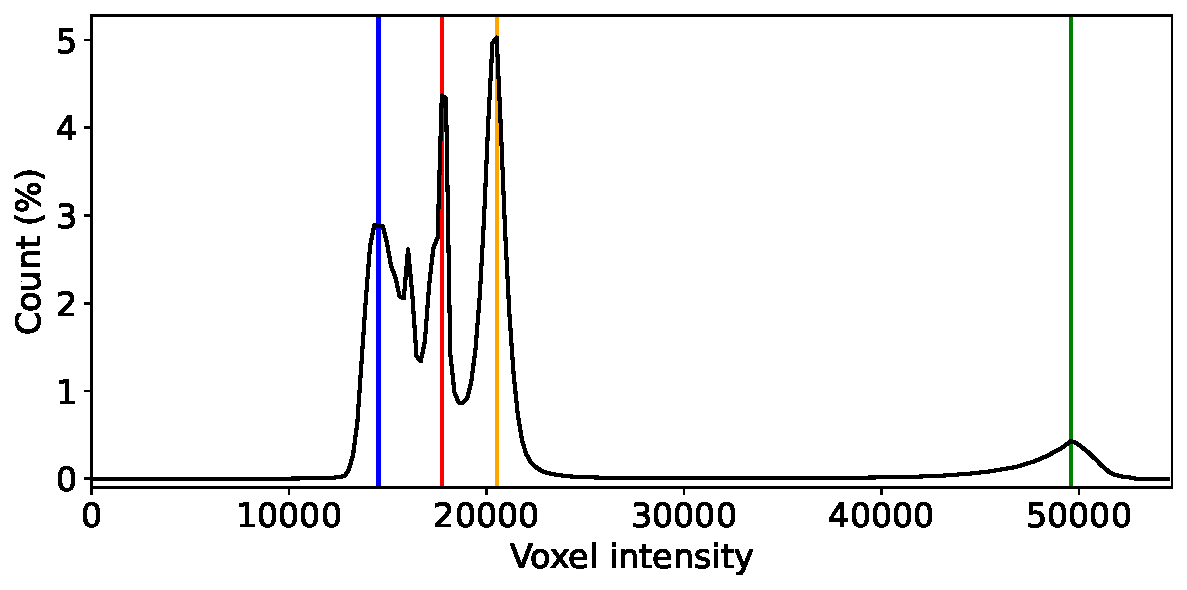
\includegraphics[width=\linewidth]{generated/770c_pag_hist_1d.pdf}
    \caption{
        1-dimensional histogram of the voxel values of an entire volume. The
        blue line is the air peak, the red line is the soft tissue peak, the
        yellow line is the bone peak, and the green line is the implant peak.
    }
    \label{fig:1d-hist}
\end{figure}

Before performing the spatially-aware segmentation analysis, we restrict the
analysis to the bone region to not expend effort on the parts of the
segmentation problem that can be solved with simpler methods.

\subsection{Computing the coarse bone region}
From the full volume, we extract the implant by globally thresholding the image
using the implant peak in the histogram, which is well-separated from the rest
of the sample. This mask is then refined by closing internal gaps followed by
finding the largest connected component, which gives us the final implant mask
visualized in \Cref{fig:bone_region} (a).

\begin{figure*}
    \centering
    \begin{tabular}{ccc}
        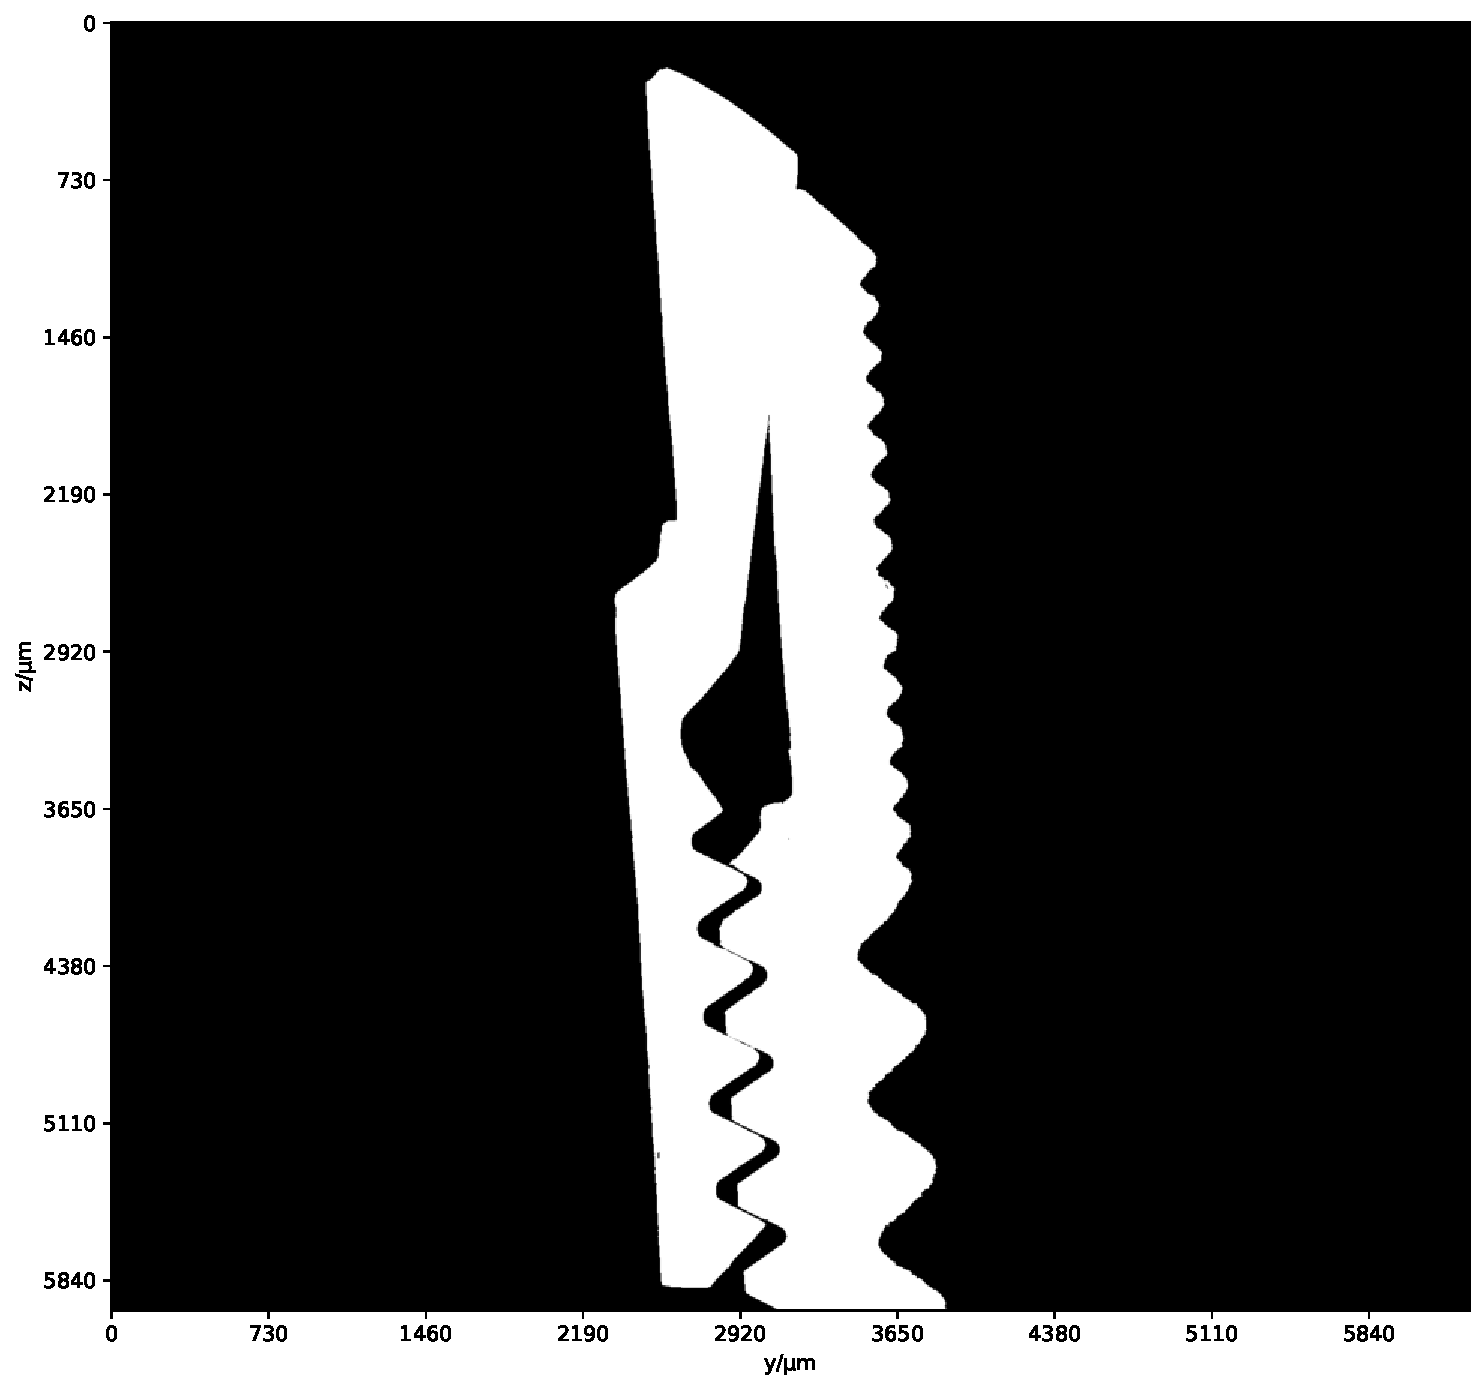
\includegraphics[width=.31\linewidth]{generated/770c_pag_mask_implant_zy.pdf} &
        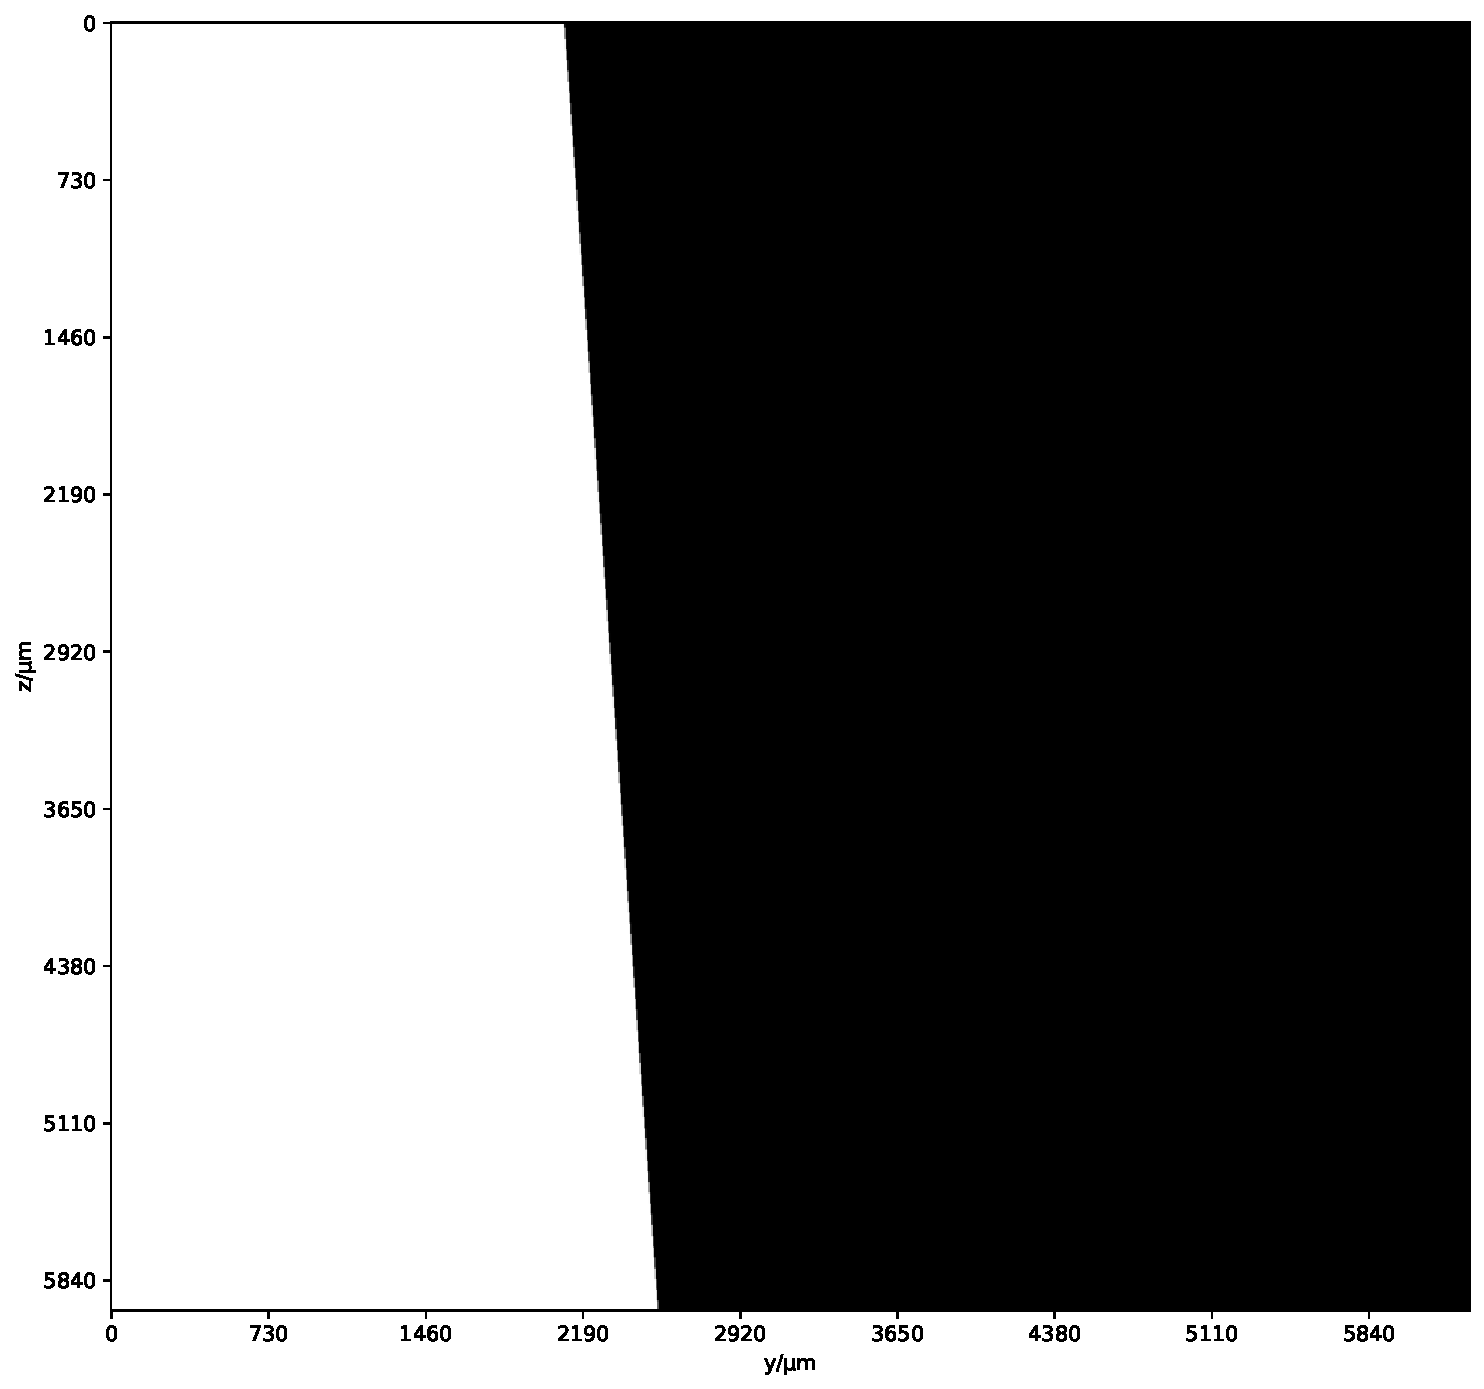
\includegraphics[width=.31\linewidth]{generated/770c_pag_mask_cut_cylinder_air_zy.pdf} &
        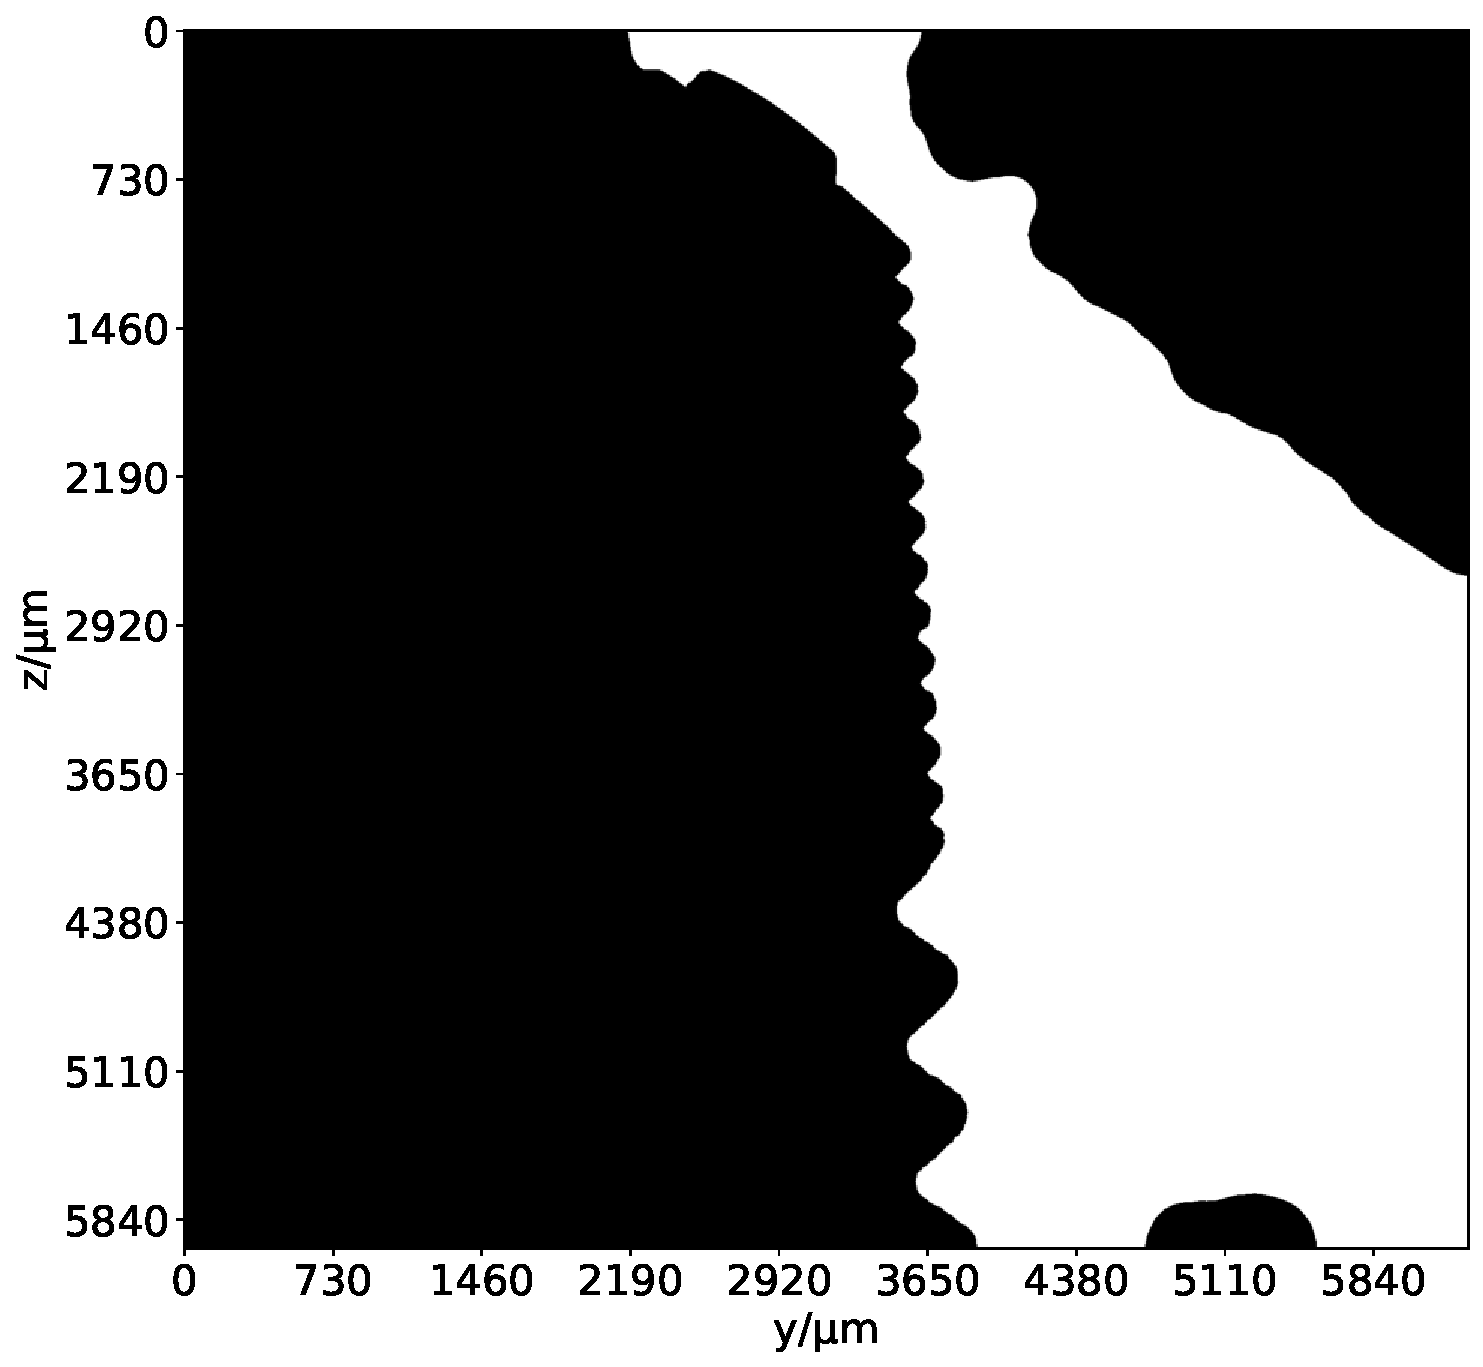
\includegraphics[width=.31\linewidth]{generated/770c_pag_mask_bone_region_zy.pdf} \\
        (a) & (b) & (c)
    \end{tabular}
    \caption{
        ZY-slices of the (a) implant mask, (b) air mask, and (c) bone region
        mask. The top blob of the bone region mask covers some of the external
        resin due to the glowing effect of the implant.
    }
    \label{fig:bone_region}
\end{figure*}

Then we remove the air depicted in \Cref{fig:3viewsample} above the implant and
to the left of the implant in the XY and YZ cross sections, respectively, as
the air introduces unwanted noise. The removal is done by computing the implant
orientation, allowing us to distinguish between the actual sample within the
cylinder and the air outside as it is facing away from the implant. This
process squashes the blue peak from the histogram, leaving the two peaks marked
by the red and orange lines as the most defined. The resulting air mask is
shown in \Cref{fig:bone_region} (b).

% We first compute a coarse bone region using a crude segmentation. Through
%direct geometric analysis of the implant, we determine the sample coordinate
%system, with the origin on the back-plane of the sawed-through implants and
%principal axes coordinate system vectors $\mathbf{u}$ pointing up towards the
%implant top, $\mathbf{v}$ pointing forward away from the back-plane, and
%$\mathbf{w}$ point right, parallel to the back-plane. An automatic
%wave-analysis of the threads computationally determines the macro-threaded
%recipient bone region, and the micro-threaded de-novo regenerated bone region.
%We then perform the spatially-aware segmentation analysis restricted to the
%bone regions to not expend effort on the parts of the segmentation
%problem that can be solved with simpler methods. Note that the process is fully
%automatic, and does not require human intervention.

As we are only interested in the voxels close to and inside the bone, and we
know that bone is the most prominent material left, we perform another coarse
segmentation by thresholding using the valley in between the two large
distributions, choosing everything to the right of this threshold as the bone
region. These voxels are then morphologically closed to consume the internal
gaps in the bone region making up the soft tissue inside the bone, followed by
morphological dilation to include the soft tissue surrounding the bone. The
resulting largest connected component is the bone region mask, which is applied
throughout subsequent steps to filter out noise in the tomography. The final
bone region mask is visualized in \Cref{fig:bone_region} (c).

\subsection{Exploiting spatial information}
Our goal is to discover how the value distributions for the different materials
change as a function of space. In other words, we wish to uncover information
about the conditional probabilities $\Pof{m}{v,\xx}$: that a voxel with value
$v$ and position $\xx$ represents material $m$. We cannot compute this directly
using only the volume, as only one voxel occupies position $\xx$.

However, if we fix one axis $x$, $y$, or $z$, the image \textit{does} contain
millions of voxels with that fixed value, enough to make good statistical
models for e.g.~the conditional probabilities $\Pof{m}{v,x}$, $\Pof{m}{v,y}$,
and $\Pof{m}{v,z}$. To this end, we compute 2D histograms that count voxel
frequencies both conditioned on value $v$ and coordinate value along either
$x$, $y$, or $z$.

To illustrate the effect of the different axes, we compute 2D histograms for
the full tomogram along the $x$, $y$, and $z$ axes, where each row in the
histogram is a 1D histogram of the voxel values along the corresponding axis.
E.g. row 20 in the $y$-2D histogram is the result of
\texttt{histogram(tomo[:,20,:])}. The 2D histograms are shown in
\Cref{fig:2dhists}, which highlights the exact effect: the peaks in the
histograms shift as we move along the ordinate of the histogram. For example,
when looking at the $y$ histogram in \Cref{fig:2dhists}(b), we see that the
rightmost line (bone) brightens (shifts right) towards the center (going
downwards) until it darkens (shifts left) again as we cross the center.
However, none of the axes $x$, $y$, or $z$ separate the materials well across
their entire range; they each capture different views of the distortions in the
tomography.

\begin{figure*}
    \centering
%    \begin{tabular}{cc}
%      \!\!\!\!\!\!(a) \begin{tabular}{c}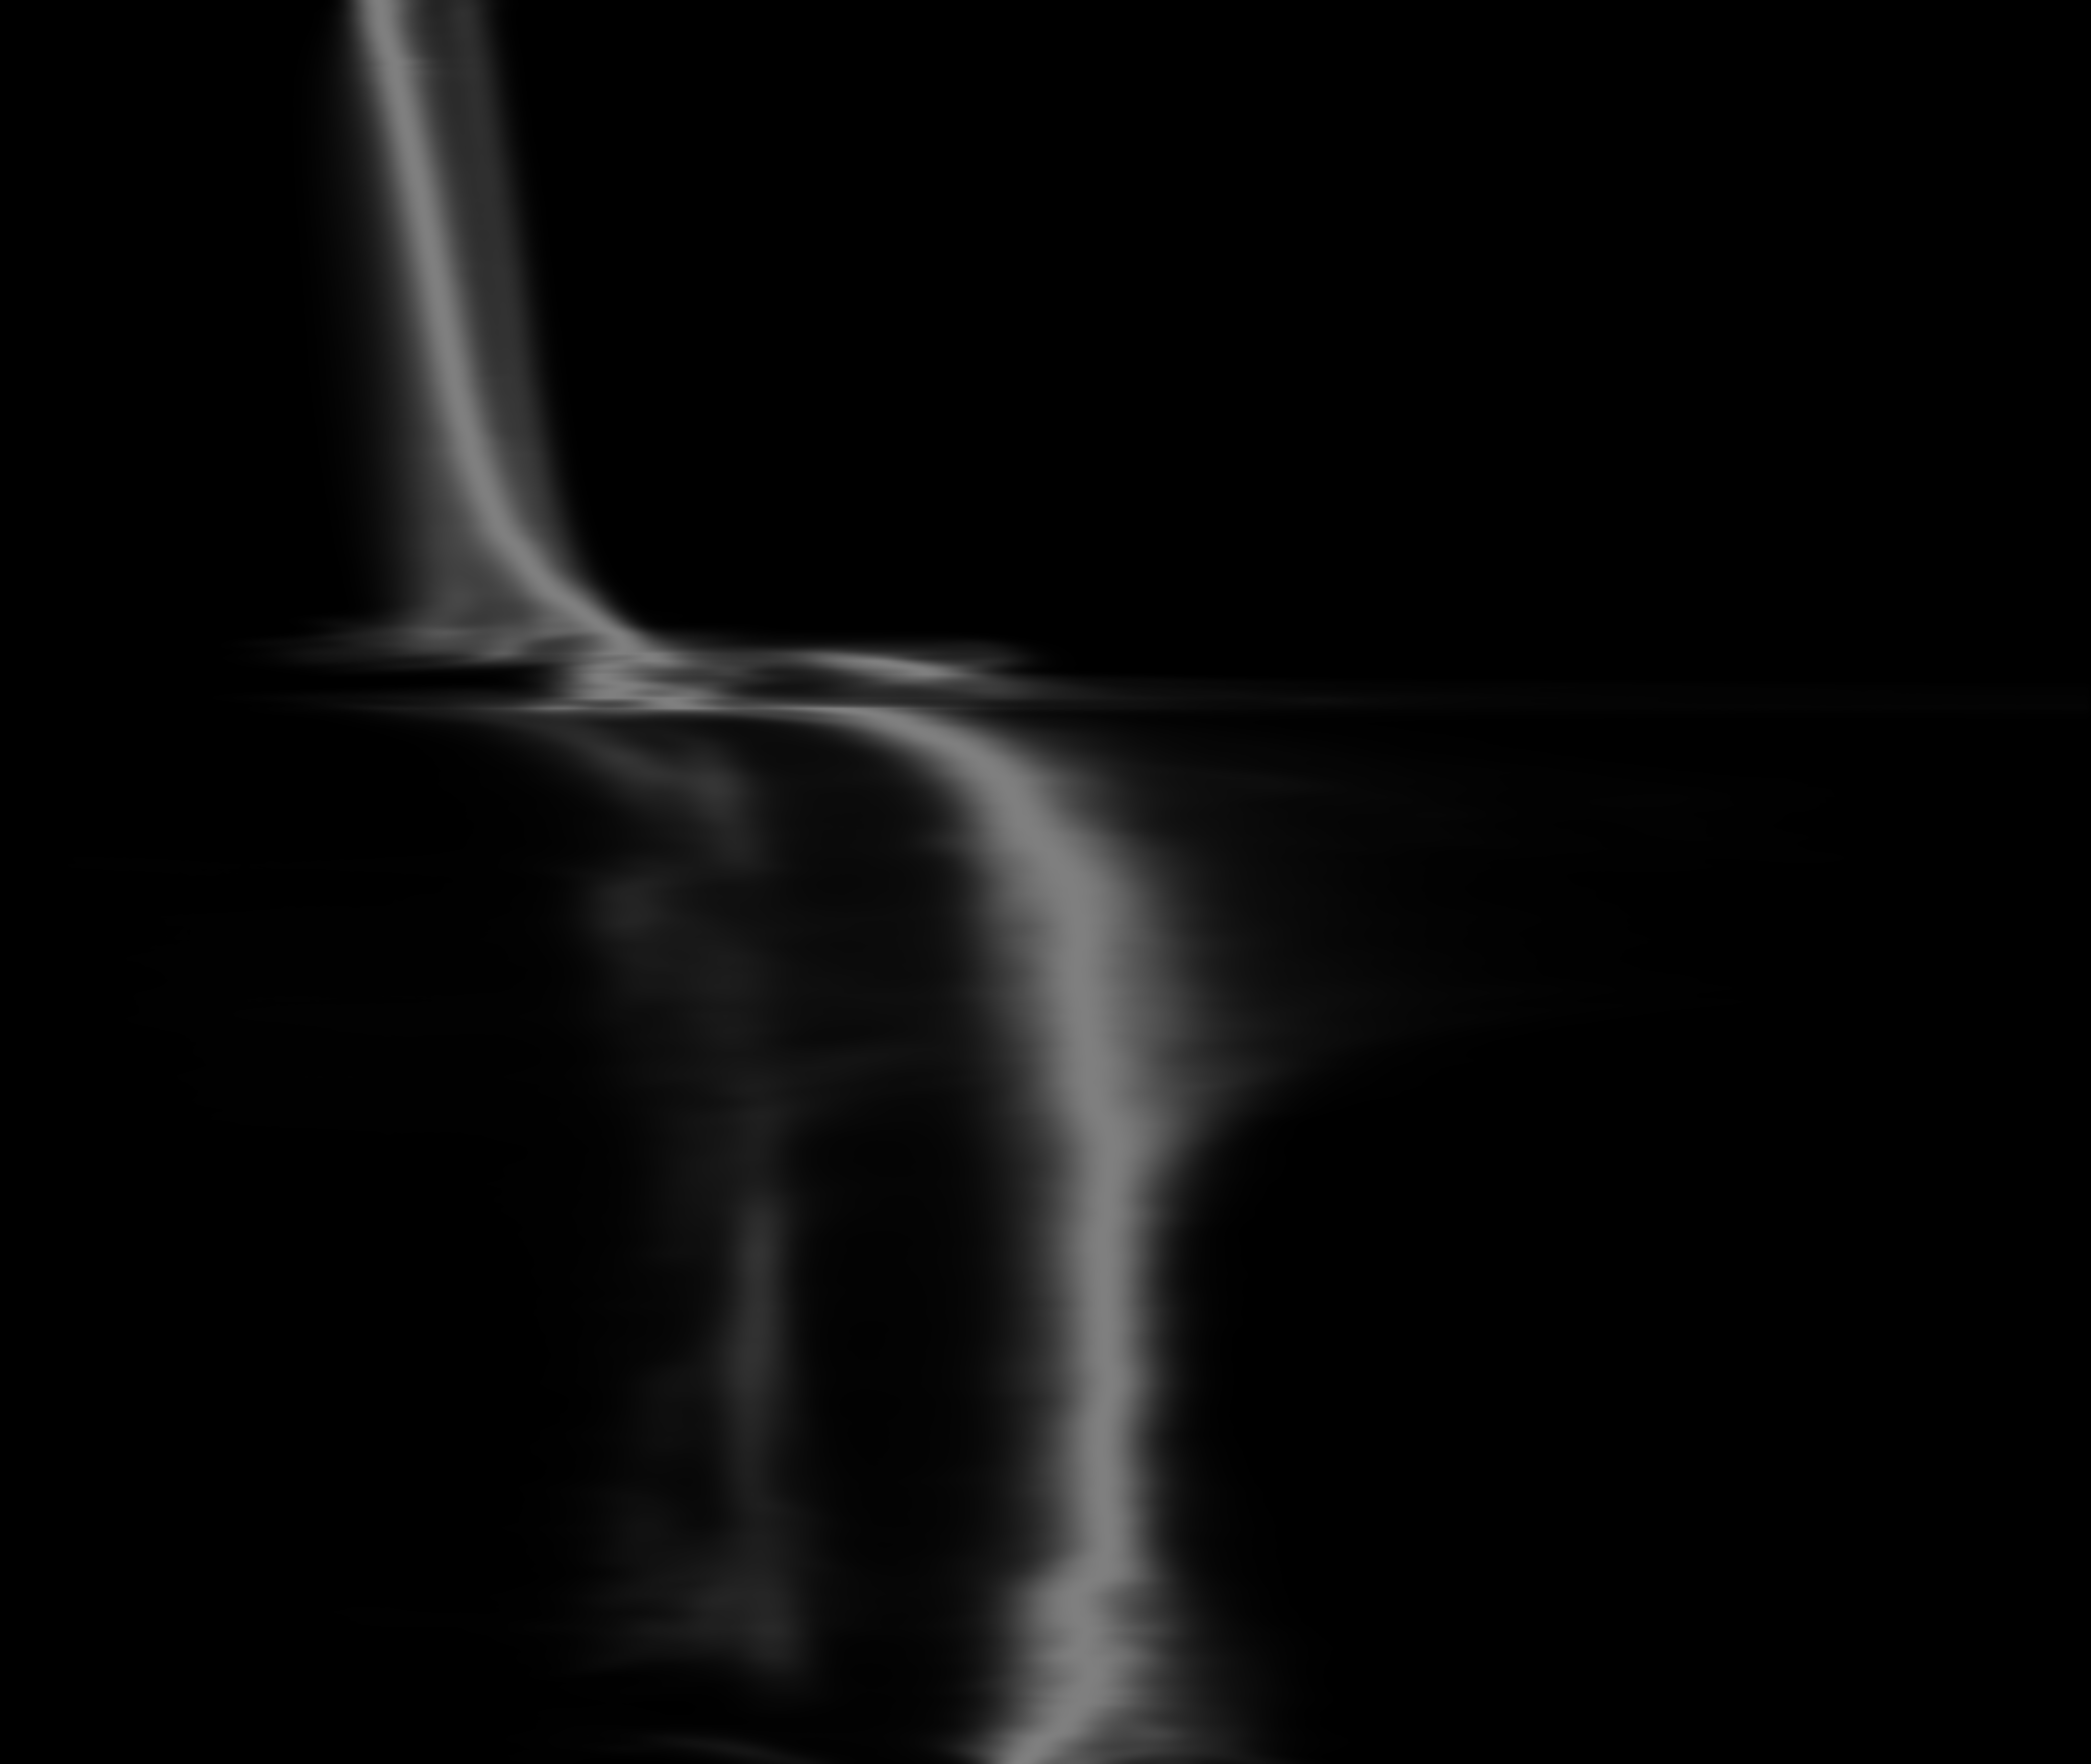
\includegraphics[width=0.7\columnwidth]{yb-full3.png}\end{tabular}\\
%      \!\!\!\!\!\!(b) \begin{tabular}{c}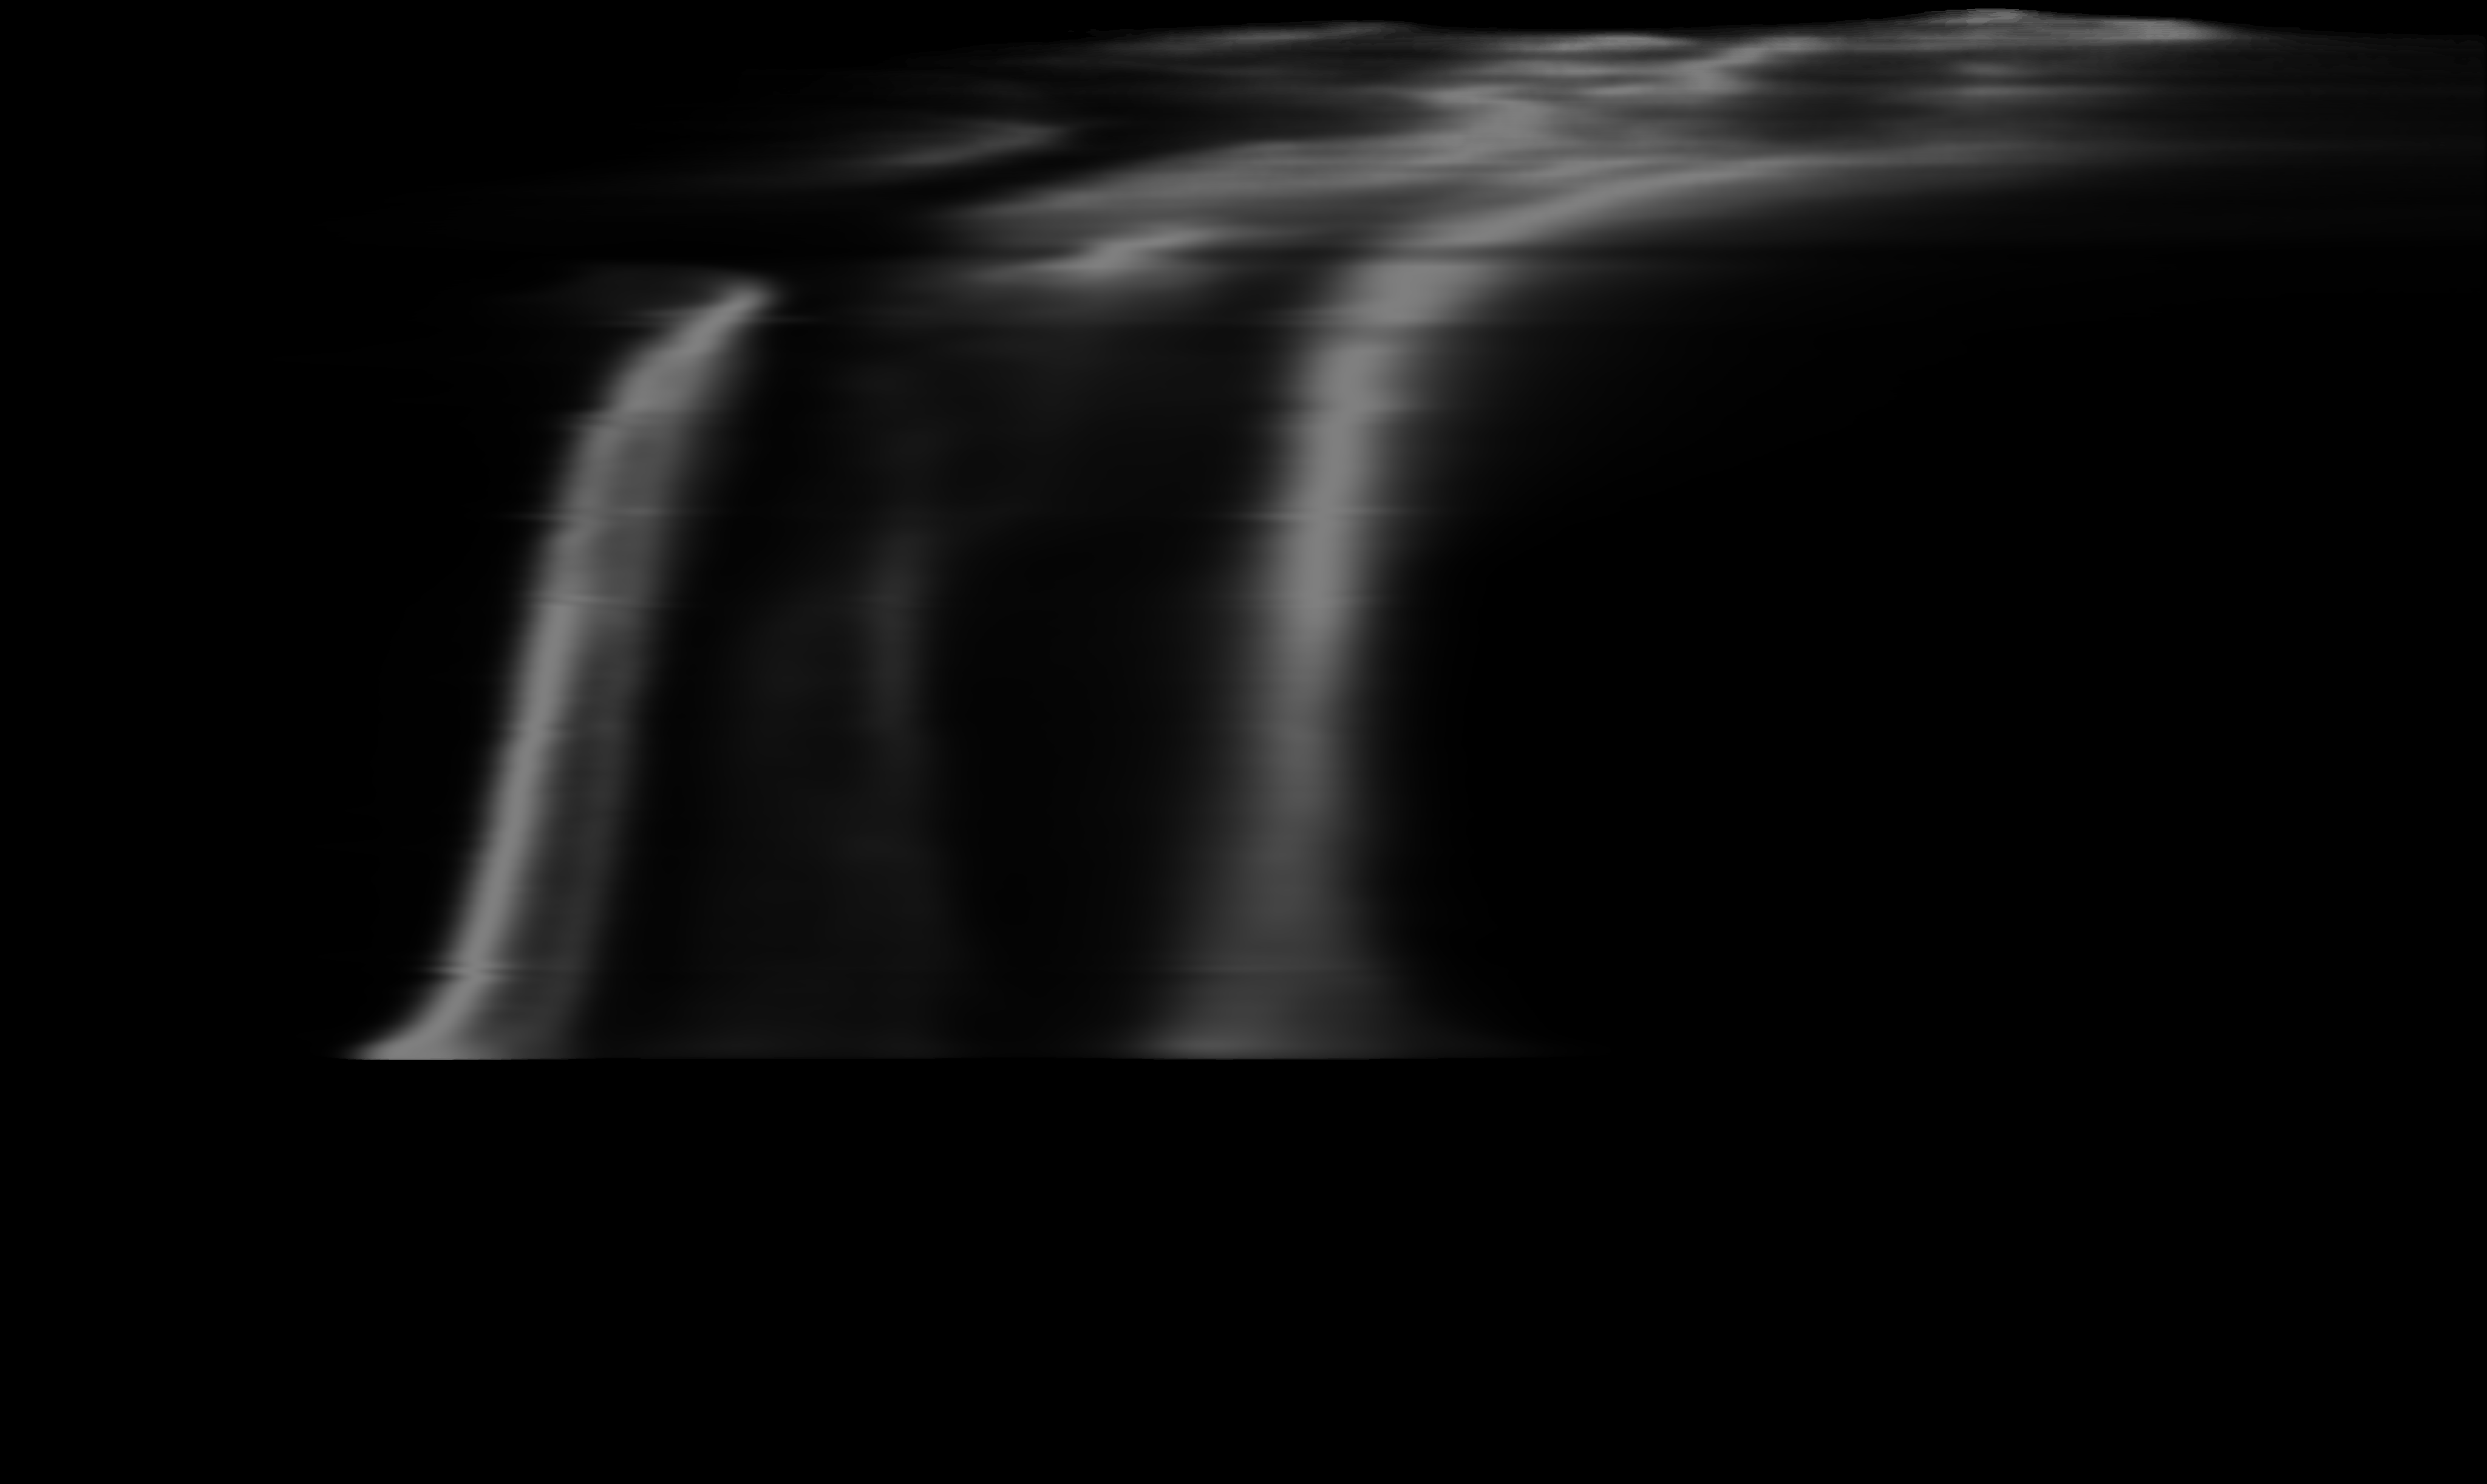
\includegraphics[width=0.7\columnwidth]{rb-full3.png}\end{tabular}\\
%      \!\!\!\!\!\!(c) \begin{tabular}{c}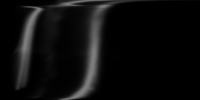
\includegraphics[width=0.7\columnwidth]{fb-edt-full2.png}\end{tabular}\\
%    \end{tabular}
    \begin{tabular}{cccc}
        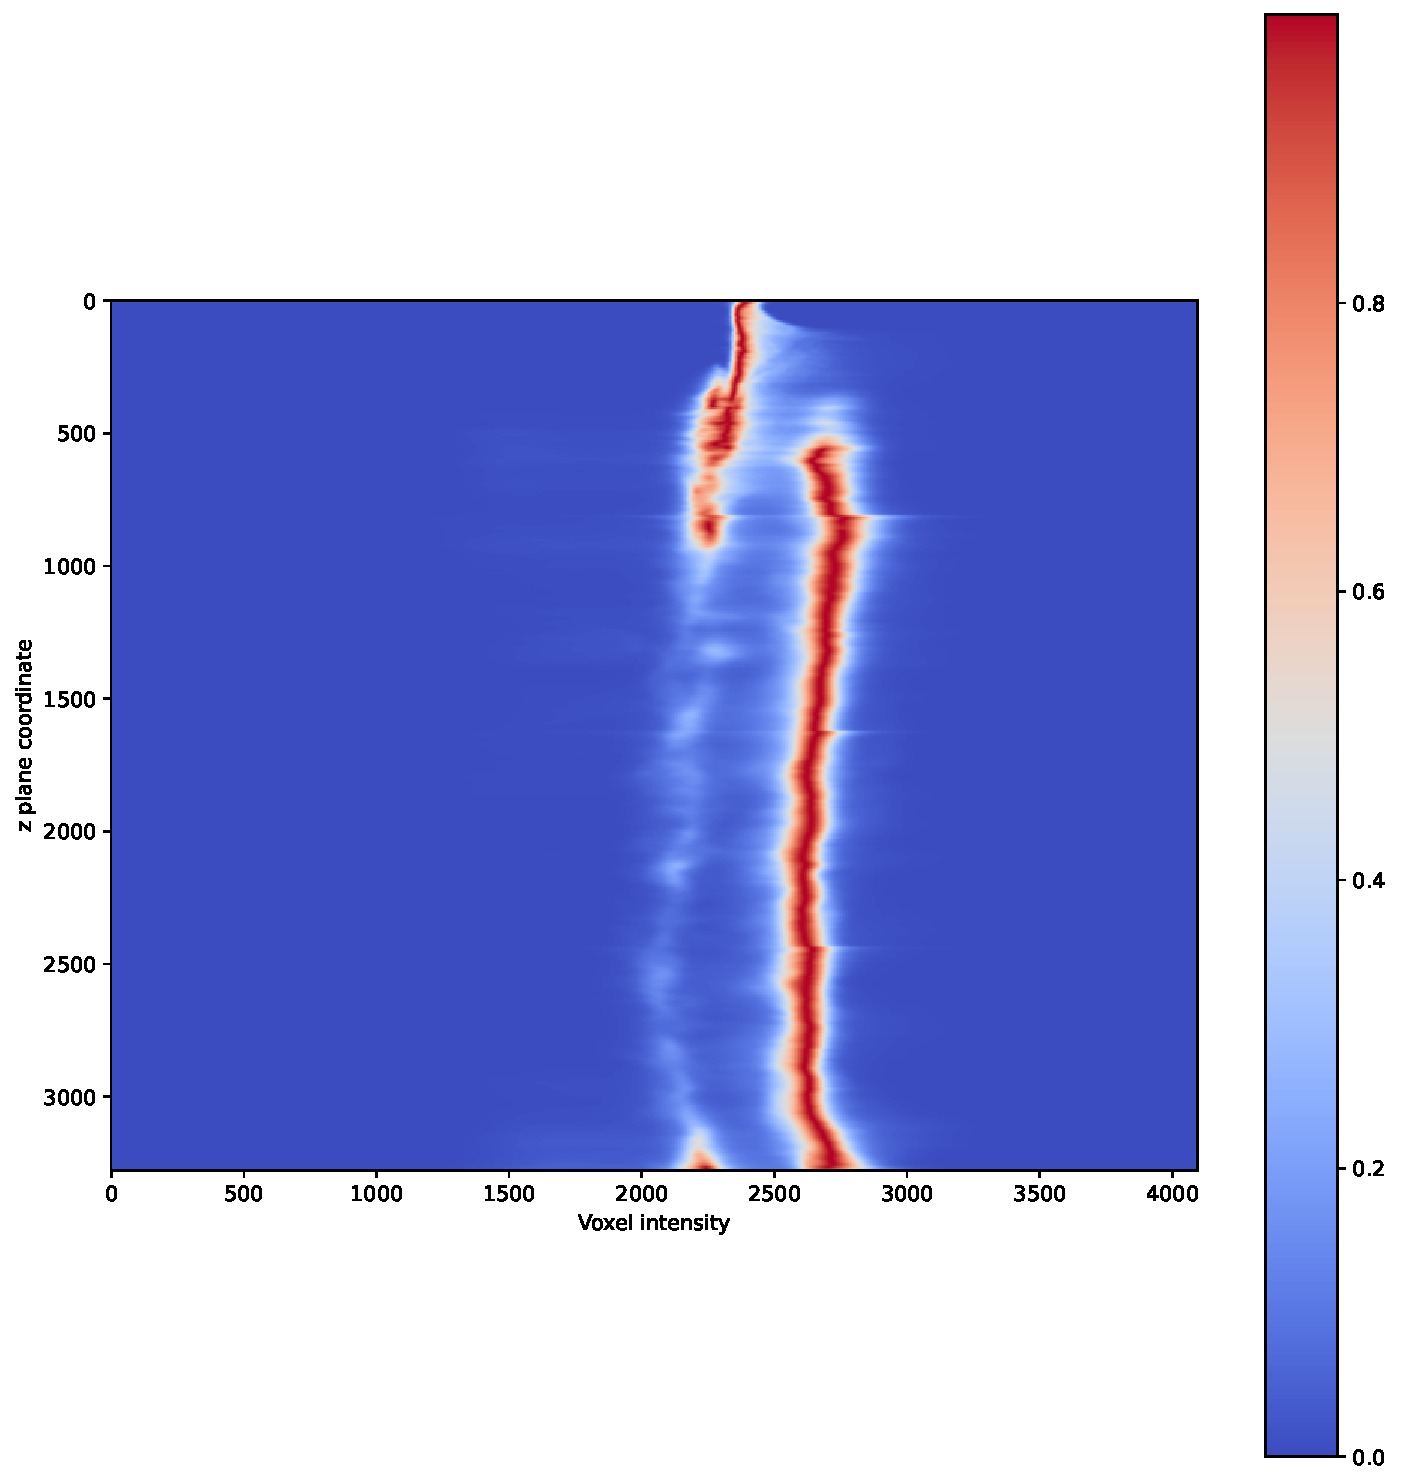
\includegraphics[width=.22\linewidth]{generated/770c_pag_hist_2d_z.pdf} &
        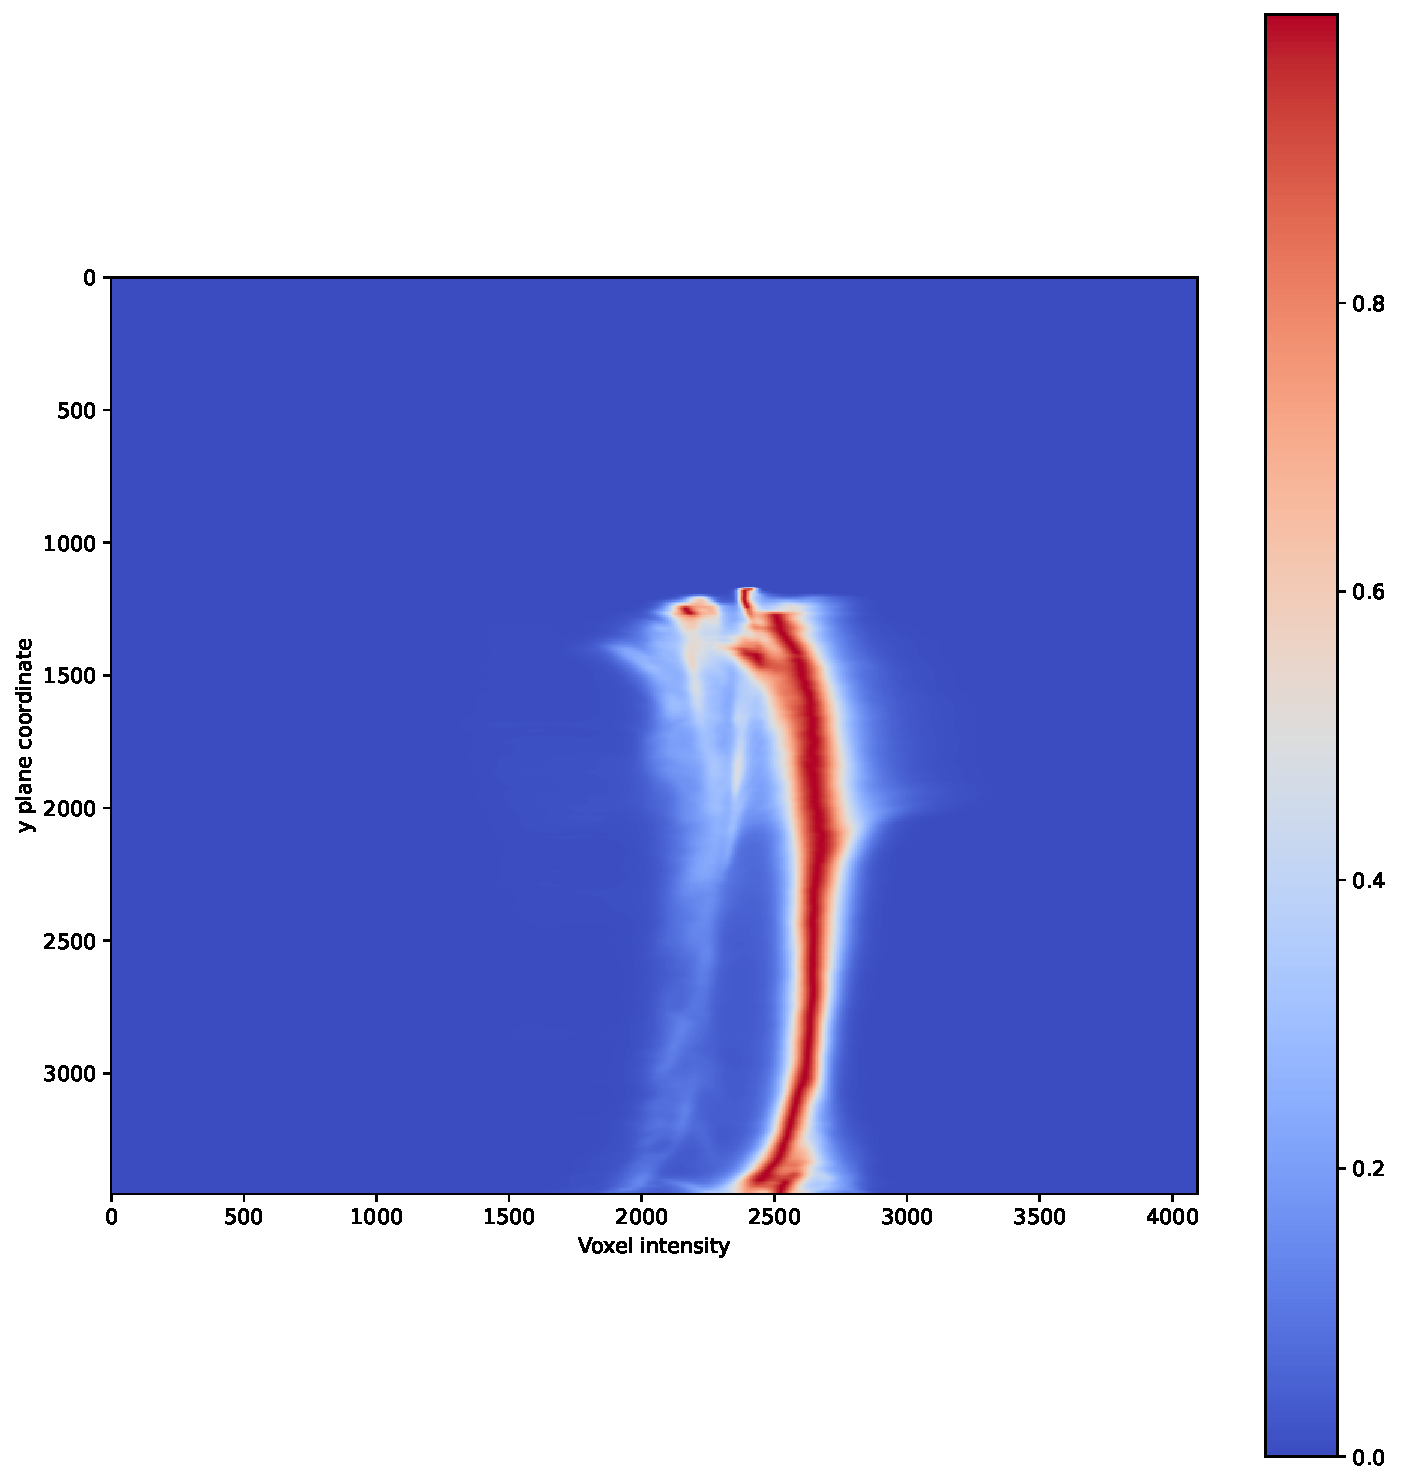
\includegraphics[width=.22\linewidth]{generated/770c_pag_hist_2d_y.pdf} &
        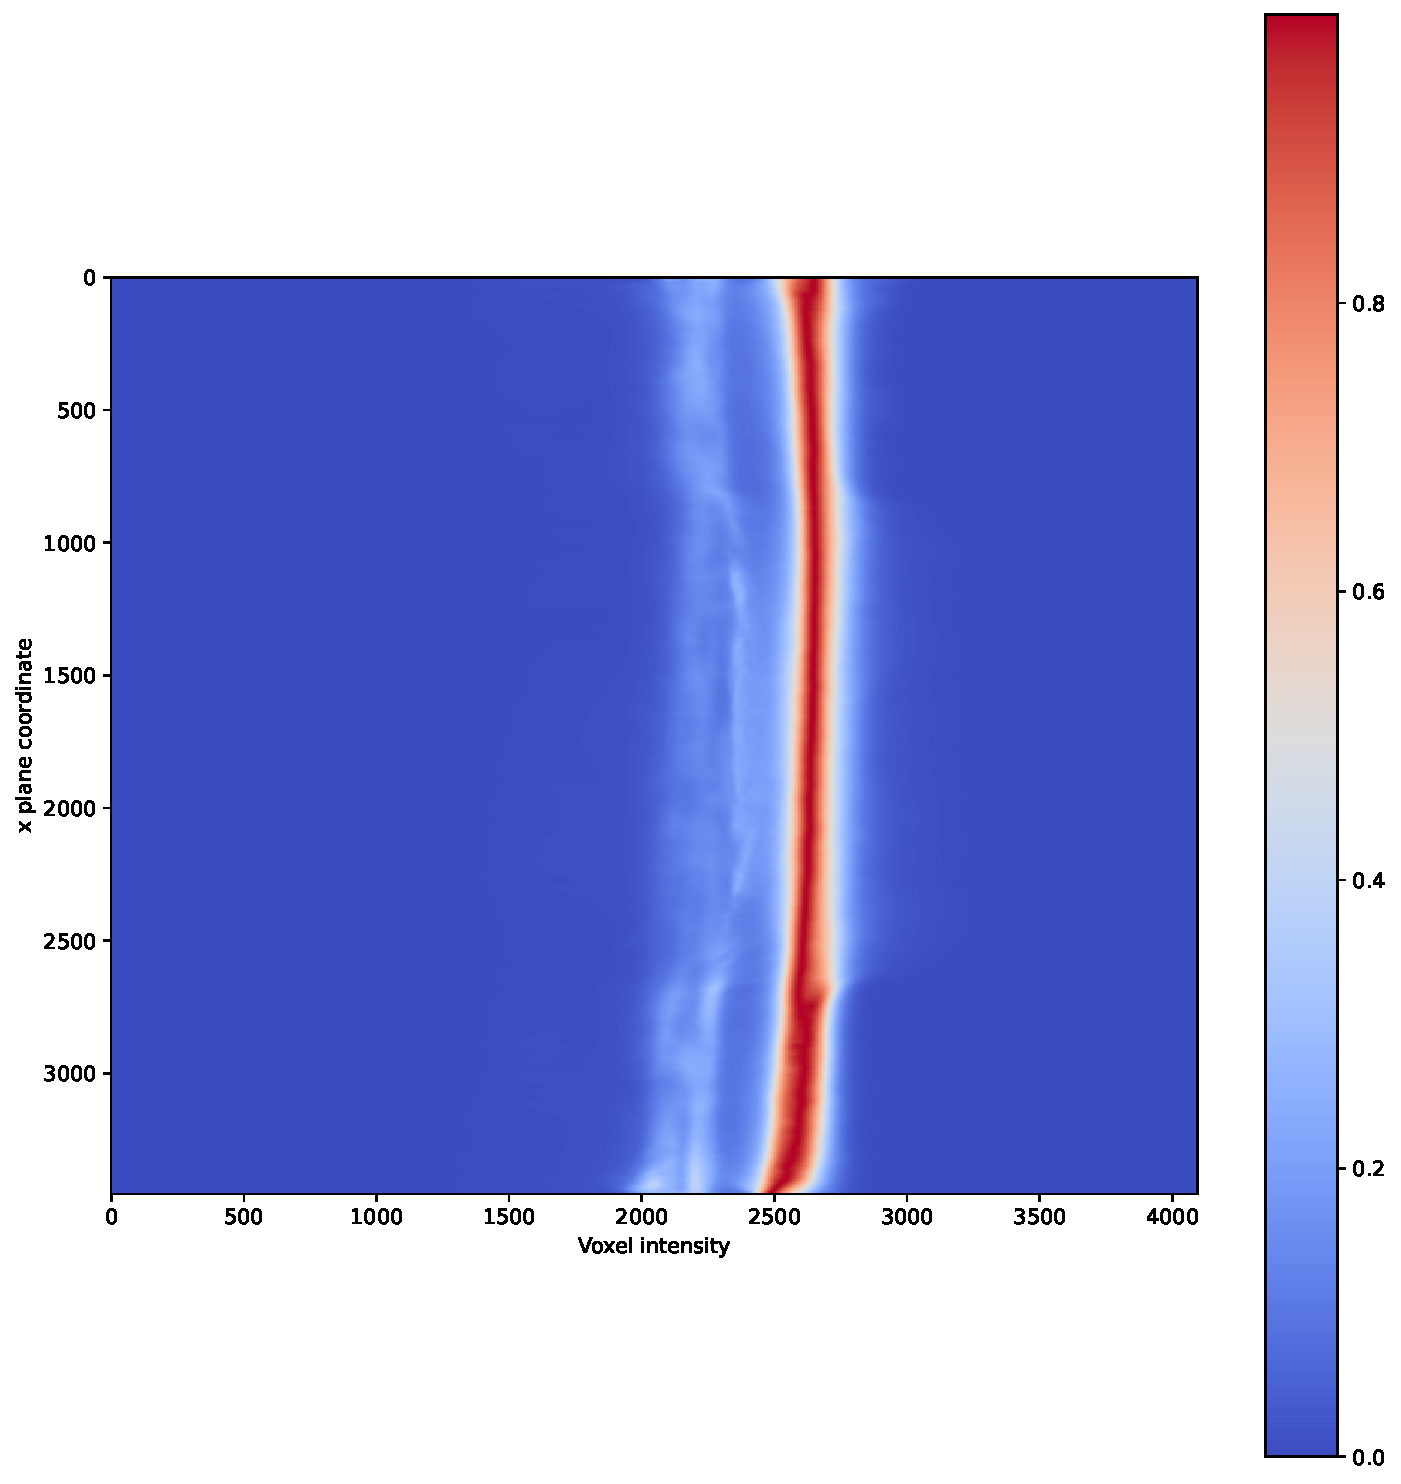
\includegraphics[width=.22\linewidth]{generated/770c_pag_hist_2d_x.pdf} &
        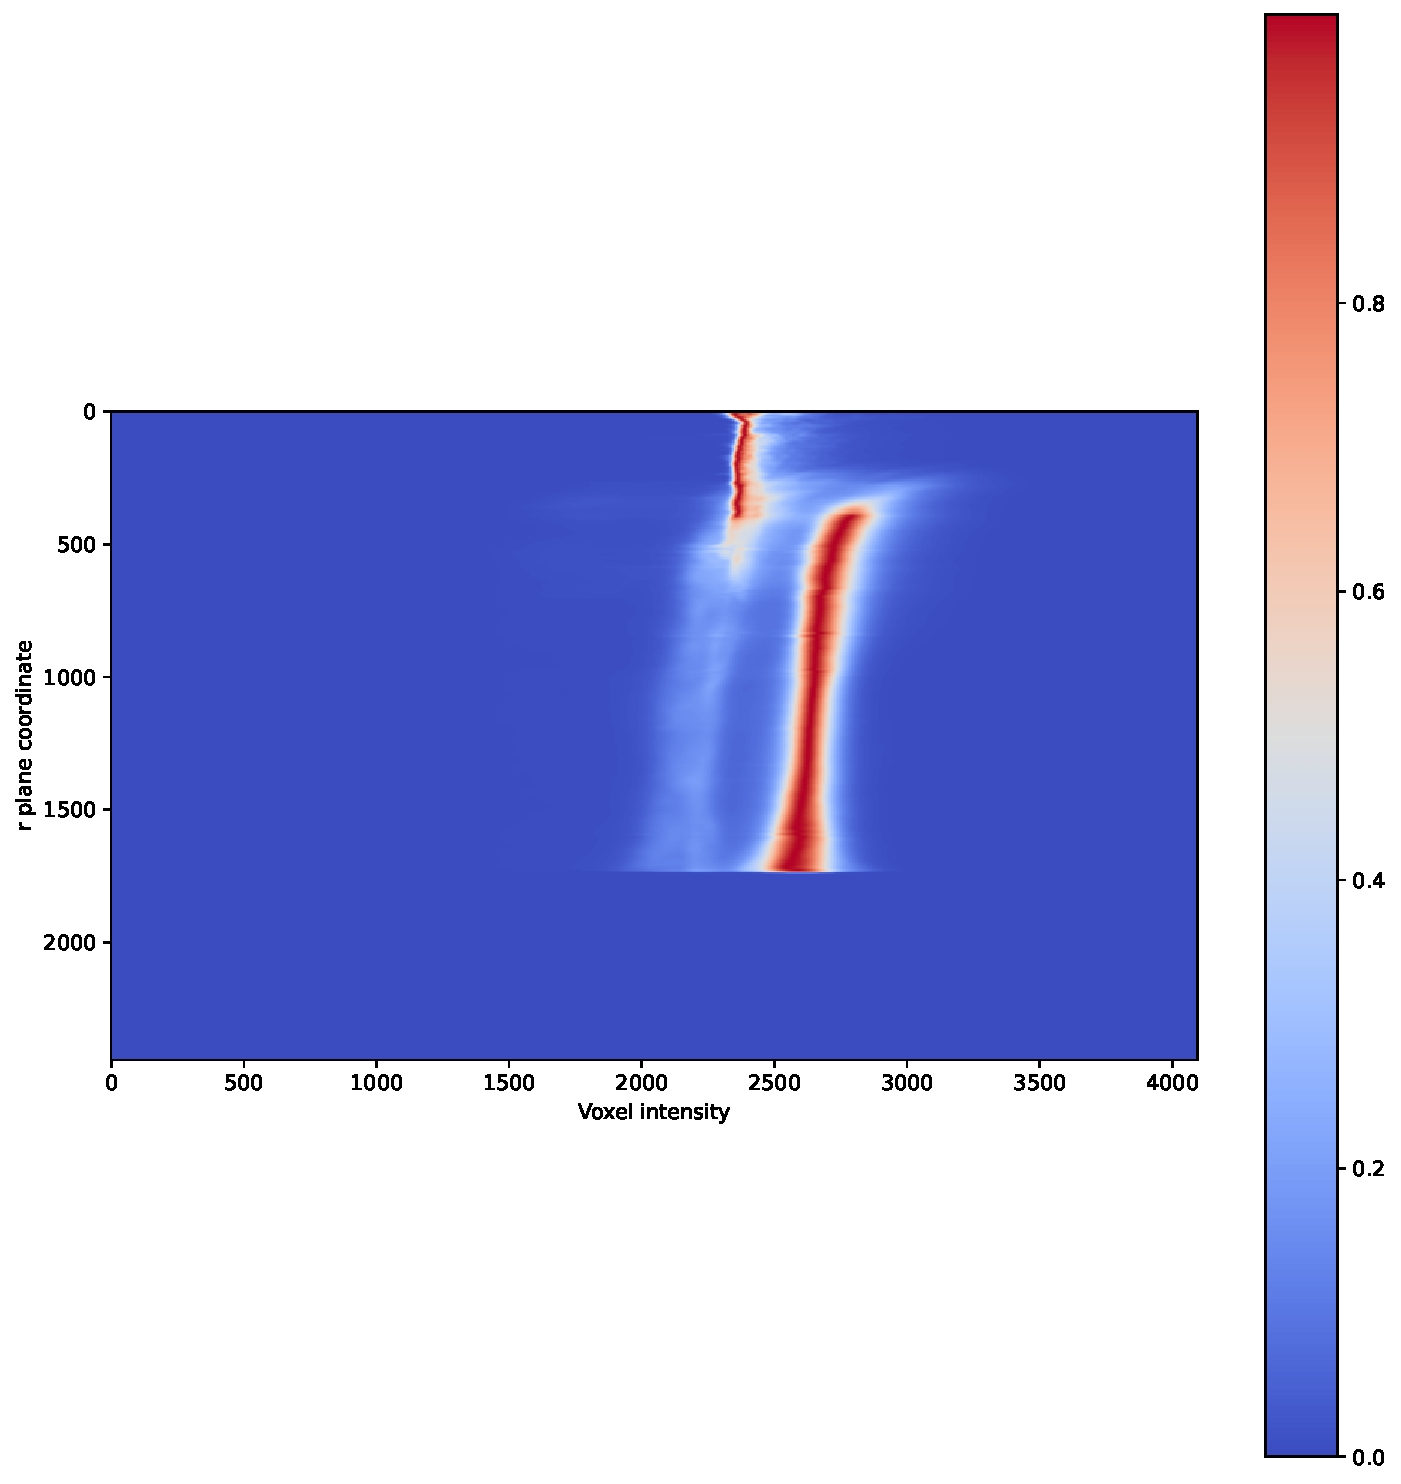
\includegraphics[width=.22\linewidth]{generated/770c_pag_hist_2d_r.pdf} \\
        (a) & (b) & (c) & (d)
    \end{tabular}
    \caption{
        2D histograms for the full volume: (a) along the $z$-axis, (b) along
        the $y$-axis, (c) along the $x$-axis, and (d) along the $r$-axis. The
        abscissa of the 2D histograms is the voxel value and the ordinate is
        the value of $z$, $y$, $x$, and $r$ respectively. Notice that the
        $r$-2D histogram well separates the materials for large and
        intermediate values of $r$, but breaks down for small $r$. However, it
        clearly shows a brightening trend for small $r$.
    }
    \label{fig:2dhists}
\end{figure*}

A better coordinate system for capturing both the distortive edge effects and
the glow from the implant is to use the cylindrical coordinates from the
tomography center line. Figure \Cref{fig:2dhists}(d) shows a similar 2D
histogram for the radial cylinder coordinate $r=\sqrt{\left(
x-c_x(z)\right)^2+\left( y-c_y(z)\right)^2}$. From this plot, we see two
prominent distributions that change along the $r$ axis. The radius correlates
with distance to the sample surface (capturing edge effects), and for medium
$r$, it is a good proxy for distance to the implant, and we see a brightening
with smaller $r$, and a darkening and broadening of the distributions for large
$r$.

Each \textit{view} provides us with additional information about how voxel
values are distorted throughout space: analogous to casting shadows along
different axes to obtain more information about a 3D object. We can either use
Bayesian statistics to combine information from multiple axes or construct a
spatial grouping that is particularly suited to capture the effects of the
distortive effects that we want to counter. The next section describes the
latter.

\subsection{Field histograms}

In the present work, the main distortion that we want to invert is the
brightening of voxels near the high-contrast interface between titanium implant
and biological tissue, to accurately determine tissue-implant contact. To this
end, we can group the voxels according to their distance from the implant using
the \textit{Euclidean Distance Transform} (EDT). \Cref{fig:fieldhists}(a) shows
the corresponding 2D histogram, which shows a darkening effect (left shift) for
large distances (bottom; near the sample surface) and brightening (right shift)
for small distances (top; the implant surface).

\begin{figure*}
    \centering
    \begin{tabular}{ccc}
        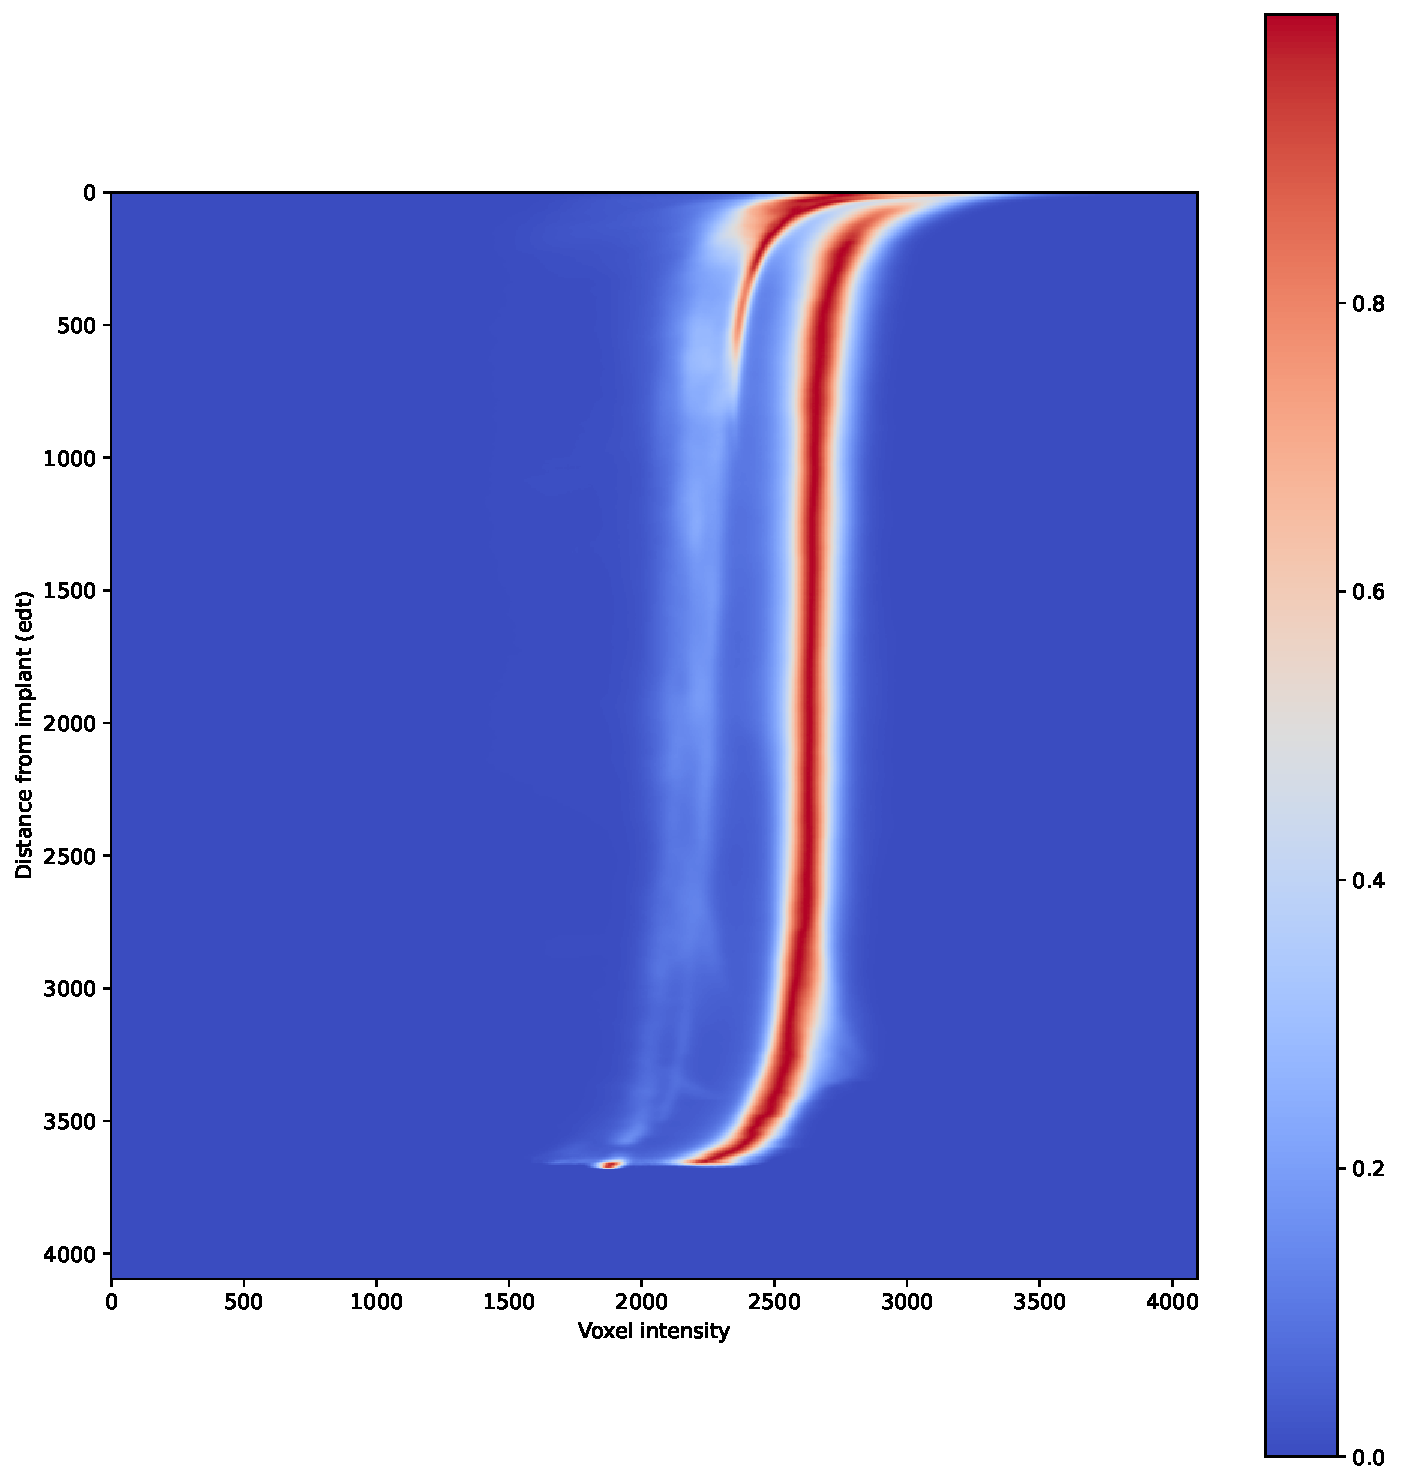
\includegraphics[width=.31\linewidth]{generated/770c_pag_hist_2d_edt.pdf} &
        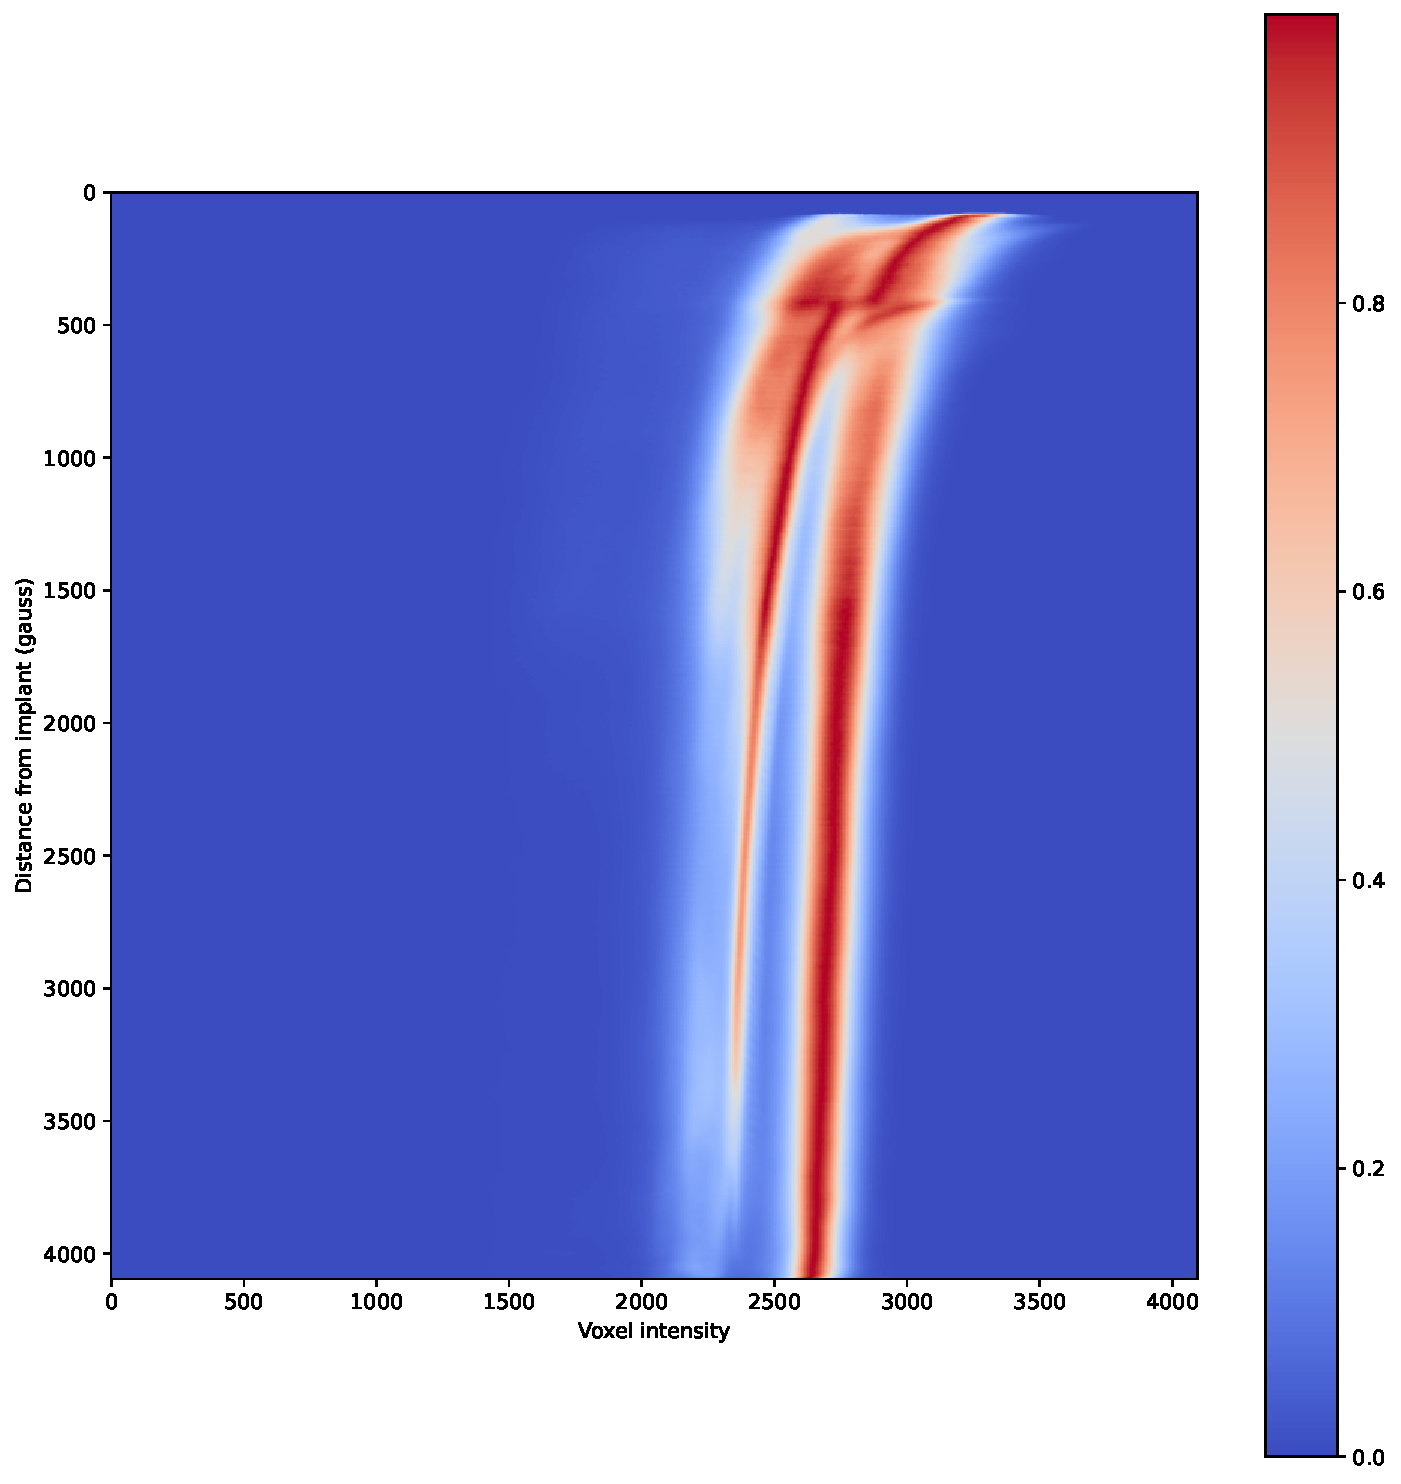
\includegraphics[width=.31\linewidth]{generated/770c_pag_hist_2d_gauss.pdf} &
        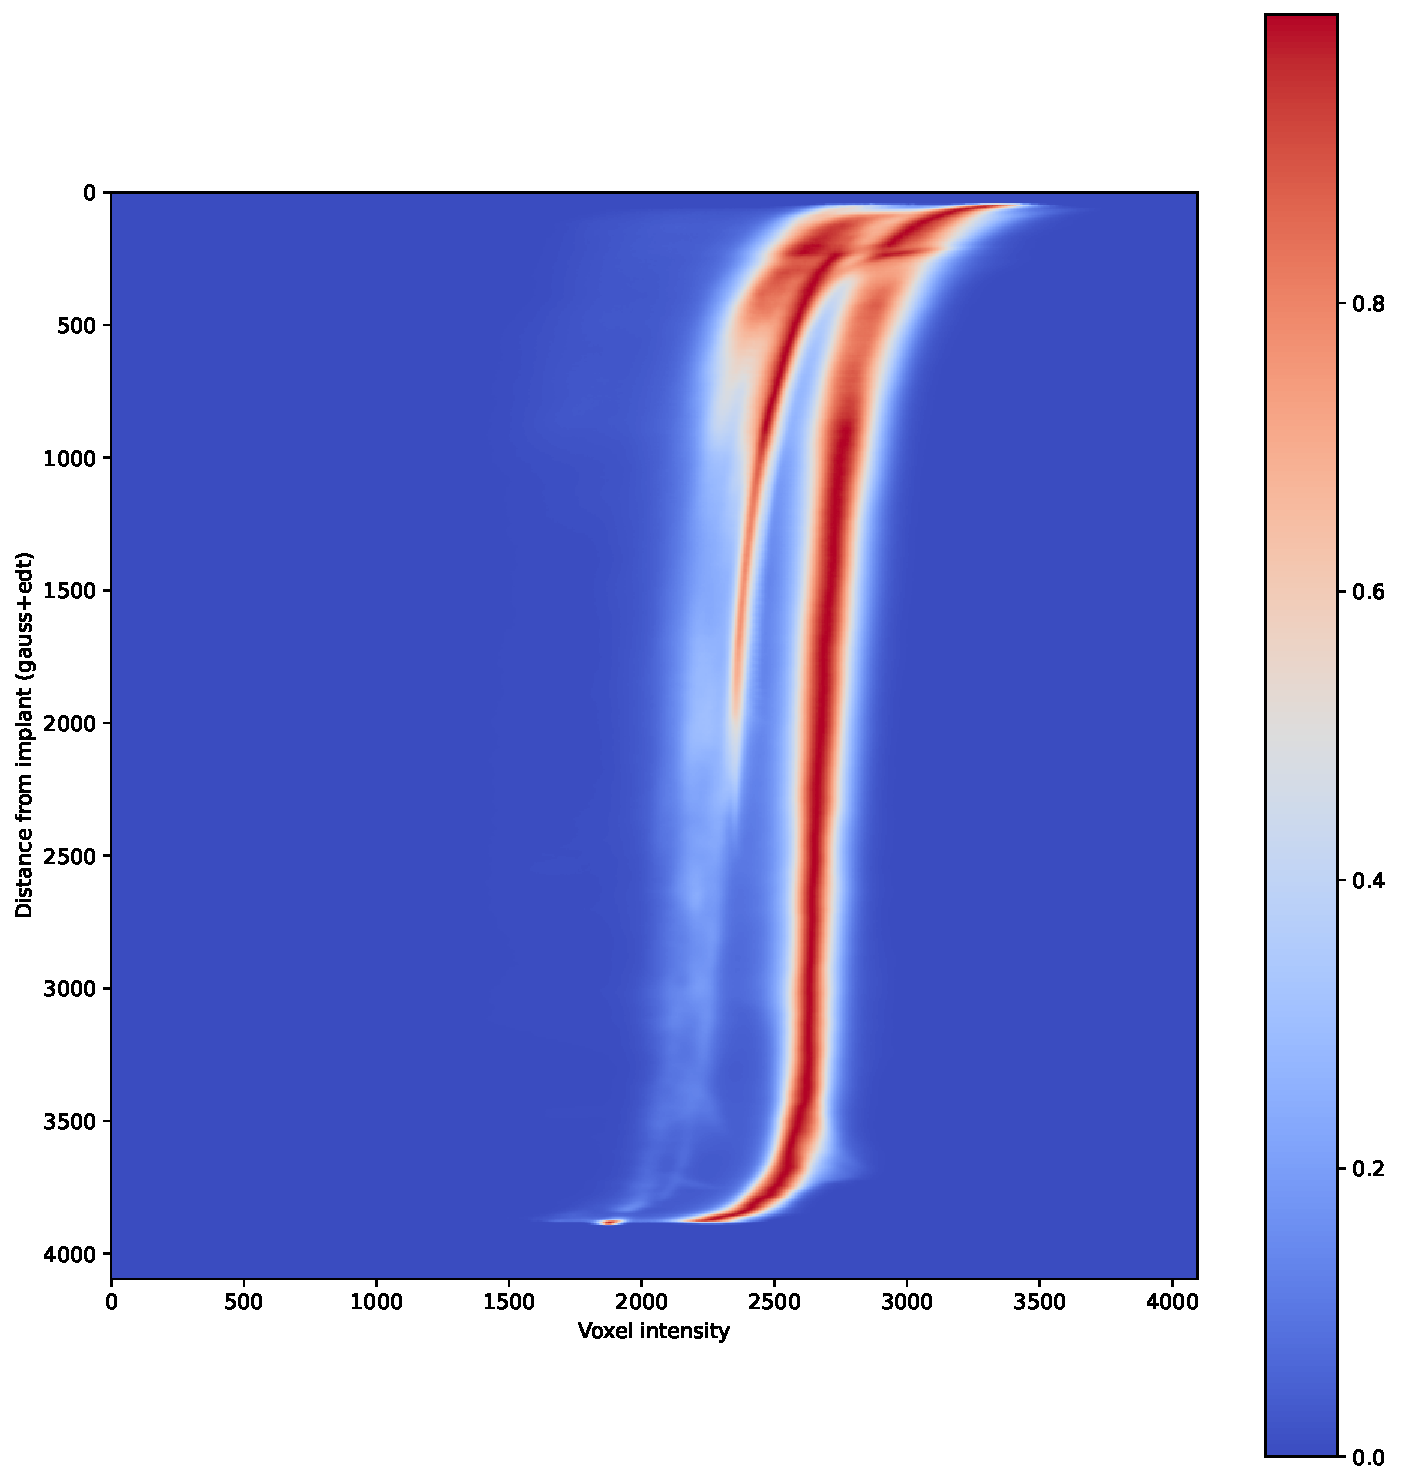
\includegraphics[width=.31\linewidth]{generated/770c_pag_hist_2d_gauss+edt.pdf} \\
        (a) & (b) & (c)
    \end{tabular}
    \caption{
        2D histogram for the field histograms: (a) EDT, (b) diffusion, and (c)
        combined. The abscissa is the voxel value and the ordinate is the field
        value - distance from the implant. The two ridges represent the
        expected value for a particular material as a function of the field
        value.
    }
    \label{fig:fieldhists}
\end{figure*}

However, we can do better: As discussed in~\Cref{sec:imaging}, the implant
produces a \textit{glowing} effect, which can be modeled physically by
diffusion. \Cref{fig:edt-vs-diffusion} shows how a voxel inside the troughs of
the threading receives brightening contributions from many sides, while a voxel
above the peak of the threading at the same distance from the implant receives
much less. To resolve the brightening of voxels very close to the implant, it
thus makes sense to use a diffusion field, as shown in \Cref{fig:field-slice},
with the corresponding 2D histogram in \Cref{fig:fieldhists}(b).

\begin{figure}
    \centering
    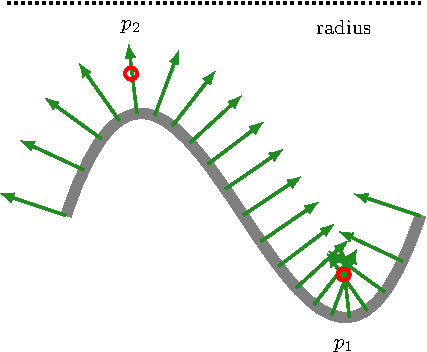
\includegraphics{figures/glowing-crop}
    \caption{
        Visualization of the glowing effect close to the implant surface, shown
        in the YZ plane. The two points $p_1$ and $p_2$, marked in red, have
        the same distance to the implant but receive a markedly different
        brightening effect. Diffusion is depicted in green, where we see
        multiple arrows contributing to the value of $p_1$. The dotted line
        depicts a constant radius from the tomogram center.
    }
    \label{fig:edt-vs-diffusion}
\end{figure}

\begin{figure}
    \centering
    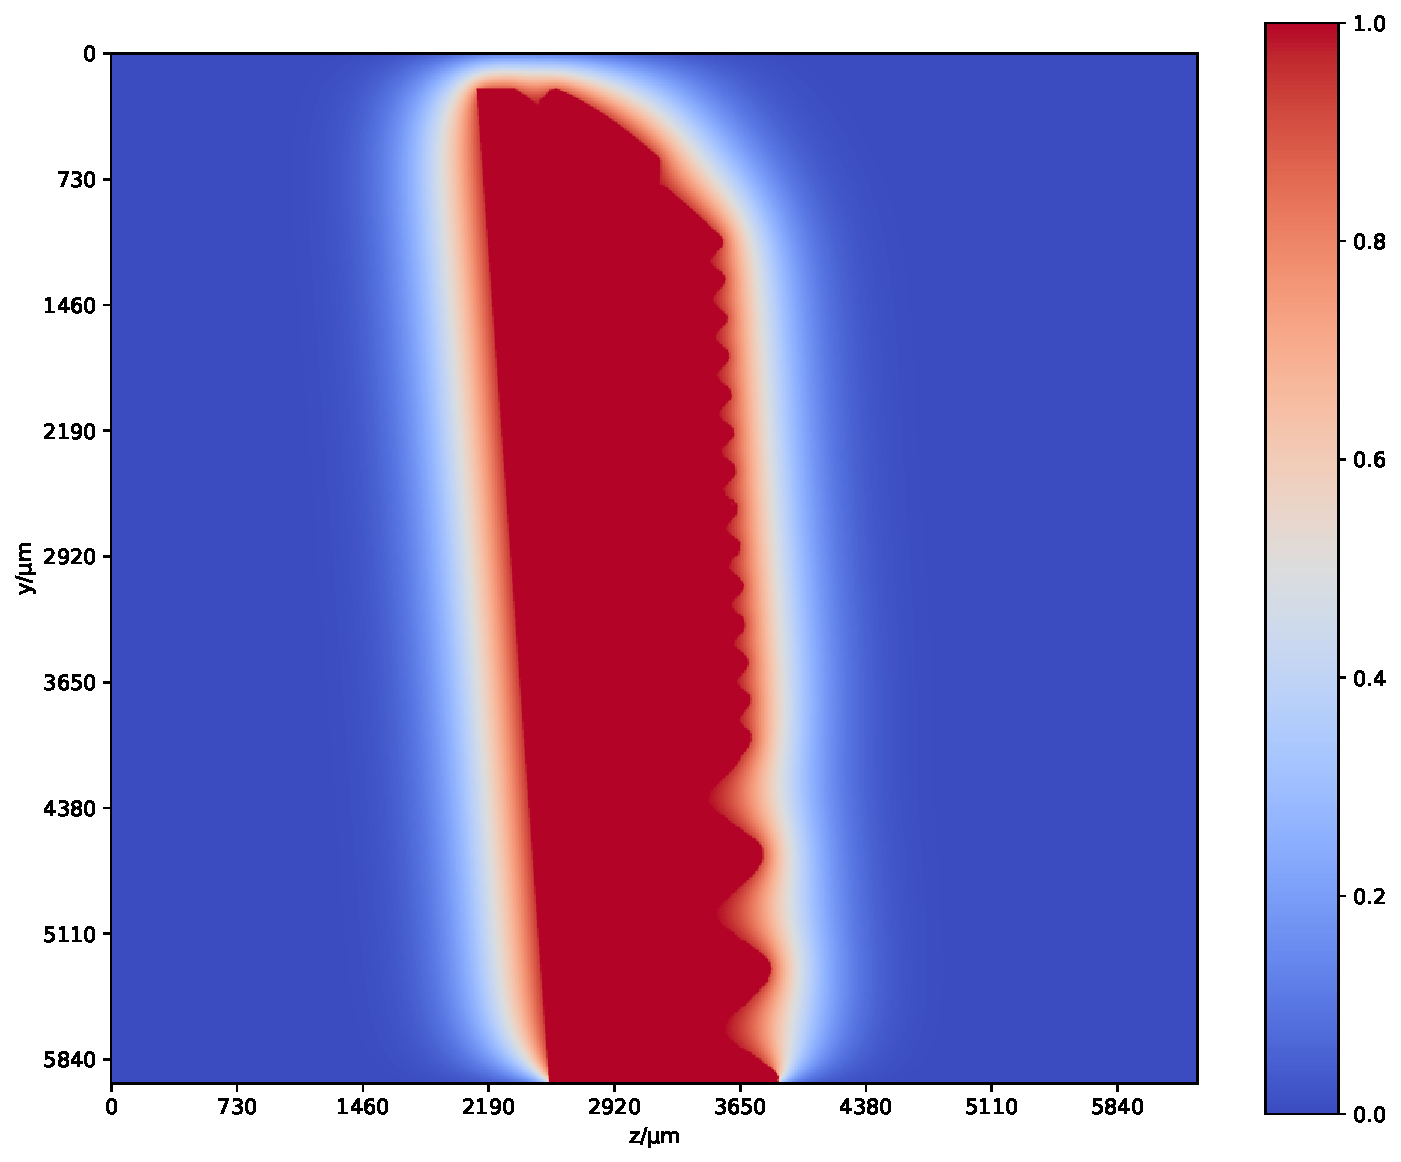
\includegraphics[width=0.75\linewidth]{generated/770c_pag_diffusion_zy.pdf}
    \caption{A slice of the diffusion field in the ZY plane.}
    \label{fig:field-slice}
\end{figure}

By using a diffusion field to model the glow from the implant, we can describe
the brightening effect even very close to the implant, but the field is nearly
zero everywhere else. To construct a single field that separates voxels well
according to the major contributions of distortion, we construct a combined
EDT+diffusion field using the procedure outlined in \Cref{eq:field-comb}.

\begin{equation}
    \label{eq:field-comb}
    \begin{split}
        f_{\text{diffusion\_norm}} &= \frac{f_{\text{diffusion}} - \min (f_{\text{diffusion}})}{\max (f_{\text{diffusion}})} \\
        f_{\text{EDT\_norm}} &= \frac{f_{\text{EDT}} - \min (f_{\text{EDT}})}{\max (f_{\text{EDT}})} \\
        f_{\text{combined}} &= f_{\text{diffusion\_norm}} - f_{\text{EDT\_norm}} \\
        f_{\text{combined\_norm}} &= \frac{f_{\text{combined}} + \|\min (f_{\text{combined}})\|}{\max (f_{\text{combined}})}
    \end{split}
\end{equation}

We will see in the next section that this histogram, shown in
\Cref{fig:fieldhists}(c), is enough to produce a high-quality segmentation
throughout the tomogram, both near the implant surface and far away from it.

\subsection{Material segmentation}

To decompose a 2D histogram into a sum of probability distributions that
represent the different materials present in the tomogram, we leverage the fact
that there are only two materials in the tomogram: bone and soft tissue. This
means we can apply classical statistical methods to separate the two materials.
For each row in the histogram, we apply Otsu's thresholding to find the
threshold that separates the two distributions best, which is shown as the
orange line in \Cref{fig:otsu}(a). This gives us a good starting point for the
segmentation, but it is not perfect as the thresholds can vary too much across
local field values.

% Continuity argument
In order for our probability distributions to be suitable for reliable
segmentation,  it is important to ensure that artifacts do in fact have a
continuous imprint.  Since the projections are acquired through rotations using
a very small step size (1/2000 of a degree) then the reconstructed volume can
be assumed to have smoothly/continuously varied features and also artifacts.
Also single projections are assumed to have continuous varying artifacts
because the projections are already heavily denoised, and it is mostly noise
which can be discontinuous. Using these probability distributions, we can build
a method to accurately identify materials across varying voxel values.

\begin{figure}
    \centering
    \begin{tabular}{cc}
        (a) & \begin{tabular}{c} 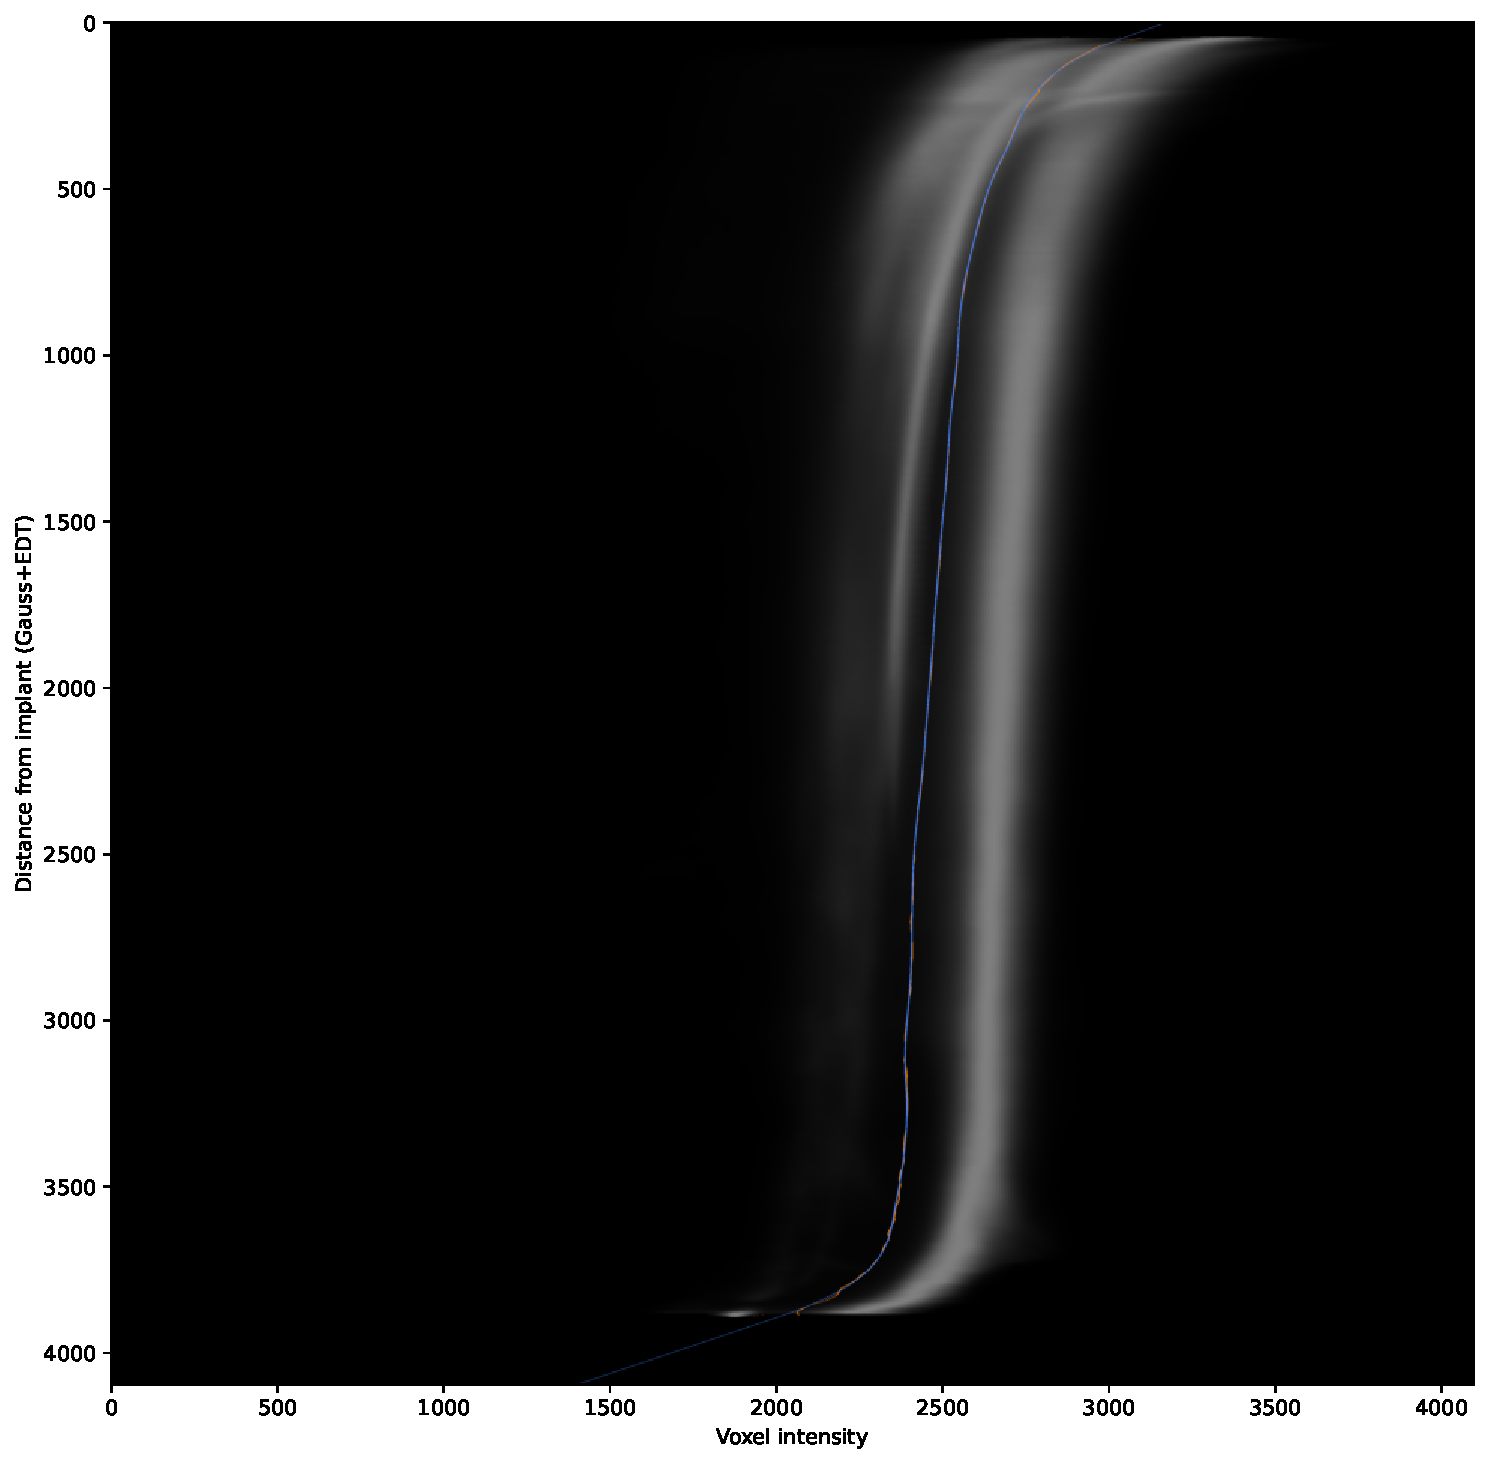
\includegraphics[width=0.8\linewidth]{generated/770c_pag_otsu.pdf} \end{tabular}\\
        (b) & \begin{tabular}{c} 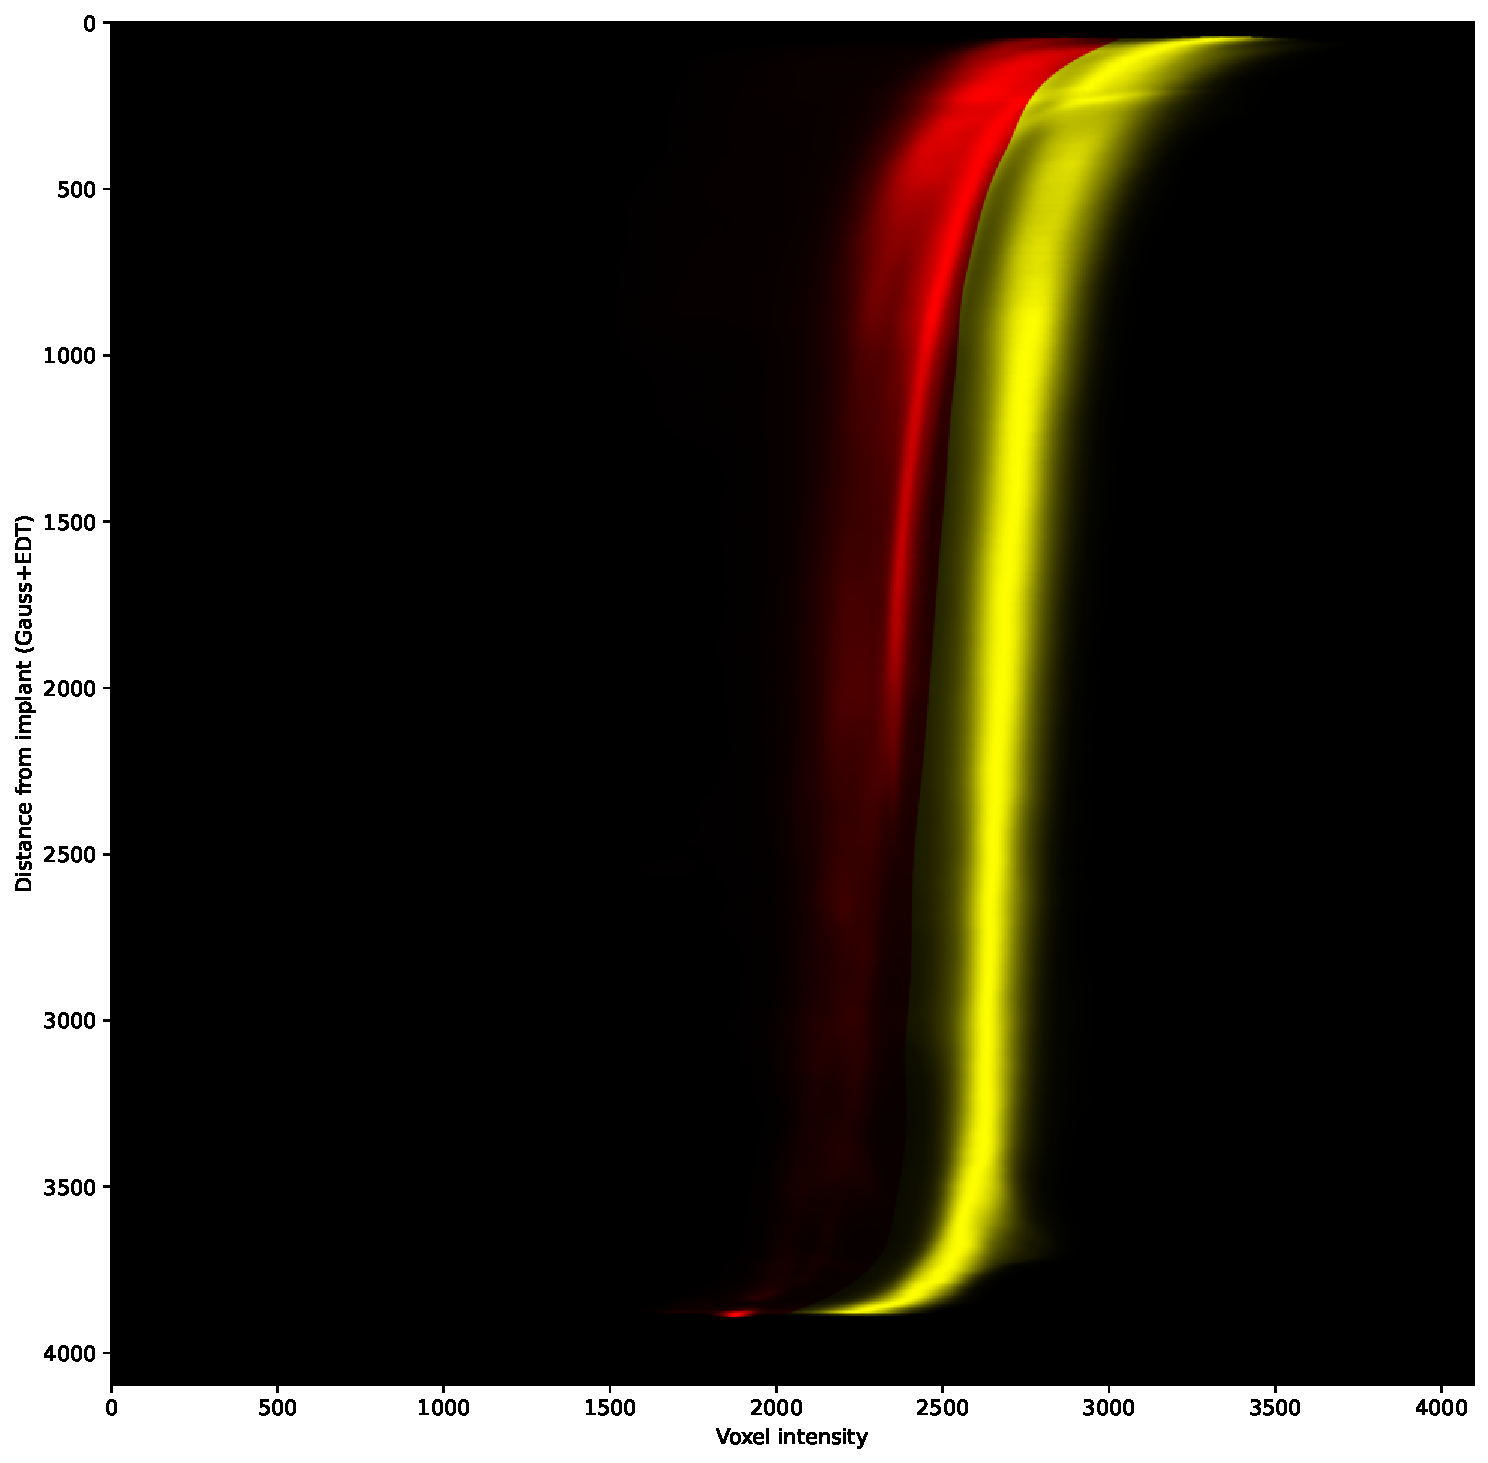
\includegraphics[width=0.8\linewidth]{generated/770c_pag_probabilities.pdf} \end{tabular}
    \end{tabular}
    \caption{
        Visualization of (a) the Otsu thresholding (orange) and the fitted
        curve (blue) applied to the combined field histogram, and (b) the
        probability distributions for the two materials, red being soft tissue
        and yellow being bone.
    }
    \label{fig:otsu}
\end{figure}

To counter this, we fit a curve to the threshold values using a piecewise cubic
function, which allows us to interpolate across the field values. This gives us
a smooth curve that separates the two materials well. This is shown in
\Cref{fig:otsu}(a) with the blue line being the fitted curve. The curve is then
used to extract the probability distributions for the two materials giving us
two mappings $P0$ and $P1$ that map the voxel value and field value to the
probability of the voxel being either bone or soft tissue. Both $P0$ and $P1$
are shown in \Cref{fig:otsu}(b). The final segmentation is then computed by
applying the mappings to the full tomogram. It is important to note that all the
steps are fully automatic and do not require any human intervention. The steps
are summarized in \Cref{fig:flowchart}.

\begin{figure}
    \centering
    %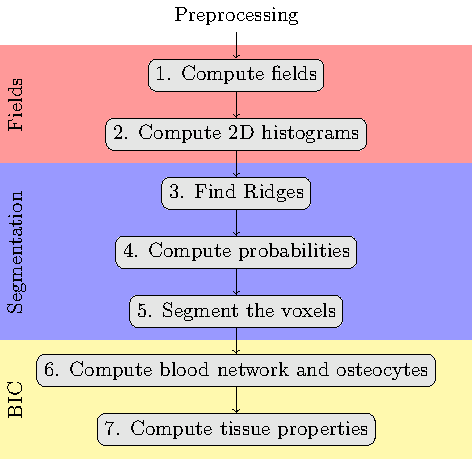
\includegraphics{steps}
    \begin{adjustbox}{width=0.6\linewidth}
        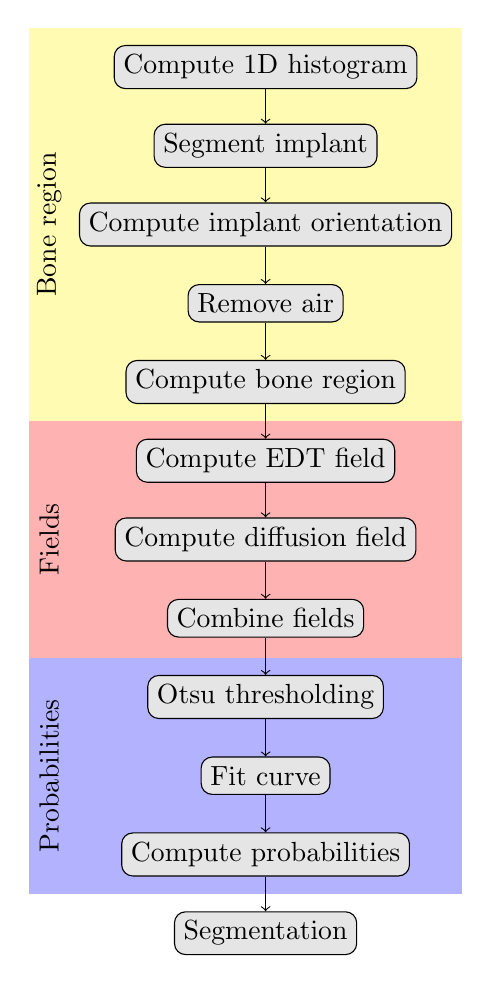
\begin{tikzpicture}
            \fill[yellow!30] (-3,-3.5) rectangle (2.5,1.5);
            \fill[red!30] (-3,-3.5) rectangle (2.5,-6.5);
            \fill[blue!30] (-3,-6.5) rectangle (2.5,-9.5);

            \node[rotate=90] (bonelab) at (-2.75,-1) {Bone region};
            \node[rotate=90] (softlab) at (-2.75,-5) {Fields};
            \node[rotate=90] (bonelab) at (-2.75,-8) {Probabilities};

            \node[draw, fill=black!10, rounded corners, rectangle] (hist1d) at (0,1) {Compute 1D histogram};
            \node[draw, fill=black!10, rounded corners, rectangle] (implant) at (0,0) {Segment implant};
            \node[draw, fill=black!10, rounded corners, rectangle] (implantfor) at (0,-1) {Compute implant orientation};
            \node[draw, fill=black!10, rounded corners, rectangle] (air) at (0,-2) {Remove air};
            \node[draw, fill=black!10, rounded corners, rectangle] (bone) at (0,-3) {Compute bone region};
            \node[draw, fill=black!10, rounded corners, rectangle] (edt) at (0,-4) {Compute EDT field};
            \node[draw, fill=black!10, rounded corners, rectangle] (diffusion) at (0,-5) {Compute diffusion field};
            \node[draw, fill=black!10, rounded corners, rectangle] (combined) at (0,-6) {Combine fields};
            \node[draw, fill=black!10, rounded corners, rectangle] (otsu) at (0,-7) {Otsu thresholding};
            \node[draw, fill=black!10, rounded corners, rectangle] (fit) at (0,-8) {Fit curve};
            \node[draw, fill=black!10, rounded corners, rectangle] (prob) at (0,-9) {Compute probabilities};
            \node[draw, fill=black!10, rounded corners, rectangle] (segment) at (0,-10) {Segmentation};

            \draw[->] (hist1d) -- (implant);
            \draw[->] (implant) -- (implantfor);
            \draw[->] (implantfor) -- (air);
            \draw[->] (air) -- (bone);
            \draw[->] (bone) -- (edt);
            \draw[->] (edt) -- (diffusion);
            \draw[->] (diffusion) -- (combined);
            \draw[->] (combined) -- (otsu);
            \draw[->] (otsu) -- (fit);
            \draw[->] (fit) -- (prob);
            \draw[->] (prob) -- (segment);
        \end{tikzpicture}
    \end{adjustbox}
    \caption{Flowchart depicting the steps of the method.}
    \label{fig:flowchart}
\end{figure}

%%% Local Variables:
%%% mode: latex
%%% TeX-master: "main"
%%% End:
